
\documentclass[journal]{IEEEtran}

% *** CITATION PACKAGES ***
%
\usepackage{cite}

% *** GRAPHICS RELATED PACKAGES ***
%
\ifCLASSINFOpdf
   \usepackage[pdftex]{graphicx}
  % declare the path(s) where your graphic files are
  % \graphicspath{{../pdf/}{../jpeg/}}
  % and their extensions so you won't have to specify these with
  % every instance of \includegraphics
 \DeclareGraphicsExtensions{.pdf,.jpeg,.png}
\else
  % or other class option (dvipsone, dvipdf, if not using dvips). graphicx
  % will default to the driver specified in the system graphics.cfg if no
  % driver is specified.
  \usepackage[dvips]{graphicx}
  % declare the path(s) where your graphic files are
  \graphicspath{{./figs/}}
  % and their extensions so you won't have to specify these with
  % every instance of \includegraphics
  \DeclareGraphicsExtensions{.eps}
\fi

% *** MATH PACKAGES ***
%
\usepackage{amsmath}


% *** SPECIALIZED LIST PACKAGES ***
%
%\usepackage{algorithmic}
% algorithmic.sty was written by Peter Williams and Rogerio Brito.
% This package provides an algorithmic environment fo describing algorithms.
% You can use the algorithmic environment in-text or within a figure
% environment to provide for a floating algorithm. Do NOT use the algorithm
% floating environment provided by algorithm.sty (by the same authors) or
% algorithm2e.sty (by Christophe Fiorio) as the IEEE does not use dedicated
% algorithm float types and packages that provide these will not provide
% correct IEEE style captions. The latest version and documentation of
% algorithmic.sty can be obtained at:
% http://www.ctan.org/pkg/algorithms
% Also of interest may be the (relatively newer and more customizable)
% algorithmicx.sty package by Szasz Janos:
% http://www.ctan.org/pkg/algorithmicx




% *** ALIGNMENT PACKAGES ***
%
%\usepackage{array}
% Frank Mittelbach's and David Carlisle's array.sty patches and improves
% the standard LaTeX2e array and tabular environments to provide better
% appearance and additional user controls. As the default LaTeX2e table
% generation code is lacking to the point of almost being broken with
% respect to the quality of the end results, all users are strongly
% advised to use an enhanced (at the very least that provided by array.sty)
% set of table tools. array.sty is already installed on most systems. The
% latest version and documentation can be obtained at:
% http://www.ctan.org/pkg/array


% IEEEtran contains the IEEEeqnarray family of commands that can be used to
% generate multiline equations as well as matrices, tables, etc., of high
% quality.




% *** SUBFIGURE PACKAGES ***
%\ifCLASSOPTIONcompsoc
%  \usepackage[caption=false,font=normalsize,labelfont=sf,textfont=sf]{subfig}
%\else
\usepackage[caption=false,font=footnotesize]{subfig}
%\fi
% subfig.sty, written by Steven Douglas Cochran, is the modern replacement
% for subfigure.sty, the latter of which is no longer maintained and is
% incompatible with some LaTeX packages including fixltx2e. However,
% subfig.sty requires and automatically loads Axel Sommerfeldt's caption.sty
% which will override IEEEtran.cls' handling of captions and this will result
% in non-IEEE style figure/table captions. To prevent this problem, be sure
% and invoke subfig.sty's "caption=false" package option (available since
% subfig.sty version 1.3, 2005/06/28) as this is will preserve IEEEtran.cls
% handling of captions.
% Note that the Computer Society format requires a larger sans serif font
% than the serif footnote size font used in traditional IEEE formatting
% and thus the need to invoke different subfig.sty package options depending
% on whether compsoc mode has been enabled.
%
% The latest version and documentation of subfig.sty can be obtained at:
% http://www.ctan.org/pkg/subfig




% *** FLOAT PACKAGES ***
%
%\usepackage{fixltx2e}
% fixltx2e, the successor to the earlier fix2col.sty, was written by
% Frank Mittelbach and David Carlisle. This package corrects a few problems
% in the LaTeX2e kernel, the most notable of which is that in current
% LaTeX2e releases, the ordering of single and double column floats is not
% guaranteed to be preserved. Thus, an unpatched LaTeX2e can allow a
% single column figure to be placed prior to an earlier double column
% figure.
% Be aware that LaTeX2e kernels dated 2015 and later have fixltx2e.sty's
% corrections already built into the system in which case a warning will
% be issued if an attempt is made to load fixltx2e.sty as it is no longer
% needed.
% The latest version and documentation can be found at:
% http://www.ctan.org/pkg/fixltx2e


%\usepackage{stfloats}
% stfloats.sty was written by Sigitas Tolusis. This package gives LaTeX2e
% the ability to do double column floats at the bottom of the page as well
% as the top. (e.g., "\begin{figure*}[!b]" is not normally possible in
% LaTeX2e). It also provides a command:
%\fnbelowfloat
% to enable the placement of footnotes below bottom floats (the standard
% LaTeX2e kernel puts them above bottom floats). This is an invasive package
% which rewrites many portions of the LaTeX2e float routines. It may not work
% with other packages that modify the LaTeX2e float routines. The latest
% version and documentation can be obtained at:
% http://www.ctan.org/pkg/stfloats
% Do not use the stfloats baselinefloat ability as the IEEE does not allow
% \baselineskip to stretch. Authors submitting work to the IEEE should note
% that the IEEE rarely uses double column equations and that authors should try
% to avoid such use. Do not be tempted to use the cuted.sty or midfloat.sty
% packages (also by Sigitas Tolusis) as the IEEE does not format its papers in
% such ways.
% Do not attempt to use stfloats with fixltx2e as they are incompatible.
% Instead, use Morten Hogholm'a dblfloatfix which combines the features
% of both fixltx2e and stfloats:
%
% \usepackage{dblfloatfix}
% The latest version can be found at:
% http://www.ctan.org/pkg/dblfloatfix




%\ifCLASSOPTIONcaptionsoff
%  \usepackage[nomarkers]{endfloat}
% \let\MYoriglatexcaption\caption
% \renewcommand{\caption}[2][\relax]{\MYoriglatexcaption[#2]{#2}}
%\fi
% endfloat.sty was written by James Darrell McCauley, Jeff Goldberg and 
% Axel Sommerfeldt. This package may be useful when used in conjunction with 
% IEEEtran.cls'  captionsoff option. Some IEEE journals/societies require that
% submissions have lists of figures/tables at the end of the paper and that
% figures/tables without any captions are placed on a page by themselves at
% the end of the document. If needed, the draftcls IEEEtran class option or
% \CLASSINPUTbaselinestretch interface can be used to increase the line
% spacing as well. Be sure and use the nomarkers option of endfloat to
% prevent endfloat from "marking" where the figures would have been placed
% in the text. The two hack lines of code above are a slight modification of
% that suggested by in the endfloat docs (section 8.4.1) to ensure that
% the full captions always appear in the list of figures/tables - even if
% the user used the short optional argument of \caption[]{}.
% IEEE papers do not typically make use of \caption[]'s optional argument,
% so this should not be an issue. A similar trick can be used to disable
% captions of packages such as subfig.sty that lack options to turn off
% the subcaptions:
% For subfig.sty:
% \let\MYorigsubfloat\subfloat
% \renewcommand{\subfloat}[2][\relax]{\MYorigsubfloat[]{#2}}
% However, the above trick will not work if both optional arguments of
% the \subfloat command are used. Furthermore, there needs to be a
% description of each subfigure *somewhere* and endfloat does not add
% subfigure captions to its list of figures. Thus, the best approach is to
% avoid the use of subfigure captions (many IEEE journals avoid them anyway)
% and instead reference/explain all the subfigures within the main caption.
% The latest version of endfloat.sty and its documentation can obtained at:
% http://www.ctan.org/pkg/endfloat
%
% The IEEEtran \ifCLASSOPTIONcaptionsoff conditional can also be used
% later in the document, say, to conditionally put the References on a 
% page by themselves.




% *** PDF, URL AND HYPERLINK PACKAGES ***
%
%\usepackage{url}
% url.sty was written by Donald Arseneau. It provides better support for
% handling and breaking URLs. url.sty is already installed on most LaTeX
% systems. The latest version and documentation can be obtained at:
% http://www.ctan.org/pkg/url
% Basically, \url{my_url_here}.




% *** Do not adjust lengths that control margins, column widths, etc. ***
% *** Do not use packages that alter fonts (such as pslatex).         ***
% There should be no need to do such things with IEEEtran.cls V1.6 and later.
% (Unless specifically asked to do so by the journal or conference you plan
% to submit to, of course. )

% correct bad hyphenation here
\hyphenation{op-tical net-works semi-conduc-tor}

\begin{document}
%
\title{Bicycle Wheel System Identification and Optimal Truing Control for Mechatronic Systems}
%
%
% author names and IEEE memberships
% note positions of commas and nonbreaking spaces ( ~ ) LaTeX will not break
% a structure at a ~ so this keeps an author's name from being broken across
% two lines.
% use \thanks{} to gain access to the first footnote area
% a separate \thanks must be used for each paragraph as LaTeX2e's \thanks
% was not built to handle multiple paragraphs
%

\author{Aaron~Hunter% <-this % stops a space
\thanks{A. Hunter is a PhD student at the Department of Computer Science and Engineering, University of California, Santa Cruz, CA, 95060 USA e-mail: aamuhunt@ucsc.edu.}% <-this % stops a space
\thanks{Manuscript received month day, year; revised month day, year.}}

% note the % following the last \IEEEmembership and also \thanks - 
% these prevent an unwanted space from occurring between the last author name
% and the end of the author line. i.e., if you had this:
% 
% \author{....lastname \thanks{...} \thanks{...} }
%^------------^------------^----Do not want these spaces!
%
% a space would be appended to the last name and could cause every name on that
% line to be shifted left slightly. This is one of those "LaTeX things". For
% instance, "\textbf{A} \textbf{B}" will typeset as "A B" not "AB". To get
% "AB" then you have to do: "\textbf{A}\textbf{B}"
% \thanks is no different in this regard, so shield the last } of each \thanks
% that ends a line with a % and do not let a space in before the next \thanks.
% Spaces after \IEEEmembership other than the last one are OK (and needed) as
% you are supposed to have spaces between the names. For what it is worth,
% this is a minor point as most people would not even notice if the said evil
% space somehow managed to creep in.



% The paper headers
\markboth{IEEE/ASME Transactions on Mechatronics,~Vol.~yy, No.~x, Month~Year}%
{Hunter \MakeLowercase{\textit{et al.}}: Bare Demo of IEEEtran.cls for IEEE Journals}
% The only time the second header will appear is for the odd numbered pages
% after the title page when using the twoside option.
% 
% *** Note that you probably will NOT want to include the author's ***
% *** name in the headers of peer review papers.                   ***
% You can use \ifCLASSOPTIONpeerreview for conditional compilation here if
% you desire.




% If you want to put a publisher's ID mark on the page you can do it like
% this:
%\IEEEpubid{0000--0000/00\$00.00~\copyright~2015 IEEE}
% Remember, if you use this you must call \IEEEpubidadjcol in the second
% column for its text to clear the IEEEpubid mark.



% use for special paper notices
%\IEEEspecialpapernotice{(Invited Paper)}

% make the title area
\maketitle

% As a general rule, do not put math, special symbols or citations
% in the abstract or keywords.
\begin{abstract}
This paper describes an \emph{in-situ} empirical modeling technique of a conventional bicycle wheel that is employed to determine the optimal tension adjustments necessary to align the wheel in lateral and radial directions while maintaining uniform tension of the spokes. The technique allows the mean tension of the spokes to be adjusted independently from variations around the mean. Additionally, a control algorithm is developed that uses lateral feedback and predicted intermediate wheel states to bring the wheel into alignment to any desired tension in a single iteration of adjustments of the tension of the spokes.  Experimental validation of the algorithm is demonstrated on a poorly tensioned and misaligned wheel summarized here:

\begin{tabular}{| l | c | c |}
    \hline
    Parameter & Inital ($\mu \pm \sigma$) & Final ($\mu \pm \sigma$)\\ \hline
    Lateral [mm] & $0.160\pm0.736$ &$-0.037\pm 0.107$ \\ \hline 
    Radial [mm] &$0.050\pm0.158$& $-0.046\pm0.047$ \\ \hline 
    Tension [N] &$556\pm211$& $1009\pm45$ \\ \hline
\end{tabular}
\end{abstract}

% Note that keywords are not normally used for peerreview papers.
\begin{IEEEkeywords}
Bicycle wheel, manufacturing, automation, modeling.
\end{IEEEkeywords}

% For peer review papers, you can put extra information on the cover
% page as needed:
% \ifCLASSOPTIONpeerreview
% \begin{center} \bfseries EDICS Category: 3-BBND \end{center}
% \fi
%
% For peerreview papers, this IEEEtran command inserts a page break and
% creates the second title. It will be ignored for other modes.
\IEEEpeerreviewmaketitle



\section{Introduction}
% The very first letter is a 2 line initial drop letter followed
% by the rest of the first word in caps.
\IEEEPARstart{T}{he} spoked bicycle wheel is one of the most ubiquitous tensioned structures in the world. While much has been written about modeling the structure itself (see \cite{FordThesis} for a comprehensive literature review) very little has been published regarding the assembly and tuning of the structure itself.  This work presents a framework for a rigorous approach to empirically modeling a bicycle wheel and provides for an optimal tensioning method for all wheels of the same type.  This framework is intended for integration into a mechatronic wheel manufacturing apparatus although the results presented here were produced by hand, albeit with the assistance of measurement sensors and a computer. 

The approach presented in this paper builds upon the one patented by Papadapolous \cite{Papadapoulos} and alluded to in \cite{HollandMech} for the wheel tensioning method. This approach is to determine the influence of a tension adjustment of each spoke on the lateral, radial and spoke tension parameters of a specific wheel.  These influence functions are placed into a model. This model is used to compute a weighted least squares estimation of the tension adjustments that minimize the wheel parameter variations for a given wheel under tensioning.  Where I improve upon previous approaches is to provide tension targeting and a method for feedback control during the tensioning process to minimize cumulative adjustment errors. 

\section{Background}
The bicycle wheel structure consists of a rim, spokes, spoke nipples, and a hub as shown in Fig(\ref{fig:geom}).  The hub anchors the spoke which is connected to the rim by a nipple threaded onto its end and seated in the rim. The wheel structure is placed under tension, which provides its stiffness and strength, by adjusting the nipples until the desired tension is achieved. Lateral stiffness of the wheel is provided by the lateral component of the spoke tension due to the spoke angles $\alpha_{nd}$ and $\alpha_d$. Lateral stiffness prevents rim warping out of the wheel plane and allows for minimization of lateral variations. Radial stiffness and compensation is provided by the radial component of the spoke tension. The optimal tension of the wheel is a balance between the two, that is, high enough tension to support the anticipated load, but below the value that begins to induce rim warpage \cite{FordThesis}. Note that there are two other degrees of freedom for rim displacements:  tangential (rim compression along the circumference) and torsion around the rim shear center.  The former acts to reduce the circumference of the rim, however, this effect is difficult to measure due to the very high stiffness of the rim in this direction.  For purposes of this work I consider the rim incompressible in the tangential direction. The latter might be of concern for wheels containing spokes significantly offset from the rim center and thus generating a twisting moment.  In this work I assume that any torsion effect is minimized when the lateral and radial variations are minimized. In practice, these effects are primarily reduced through appropriate rim design.

Spoking patterns vary from purely radial to nearly tangential relative to the hub and determined by angle $\beta$.  Tangential spoke patterns allow for torque transmission from the hub to the rim, which occurs through the drive train or from disc brakes.  With the exception of front wheels for use with rim brakes most wheels are built with some amount of tangential spoking. 

The process of adjusting the tension to minimize the lateral and radial variations of the wheel is called truing. The typical procedure for wheel truing by hand is a heuristic where first some average spoke tension is applied by tightening all the spoke nipples, then the lateral variations are iteratively reduced, and finally the radial variations are minimized. The wheel tension is then increased incrementally and the procedure is repeated until the wheel parameter specifications are met \cite{Brandt}.

The wheel can be modeled as a system of springs operating in a linear regime \cite{FordThesis}. Because of this linear property, the wheel parameter variations induced by changes in the spoke tensions can be decomposed into the changes induced by each spoke and superposed, lending itself to influence matrix approach developed later in this work.

\begin{figure}[!t]
\centering
    \subfloat[]{
        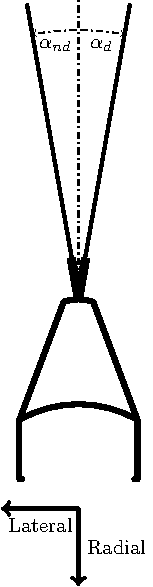
\includegraphics[width=0.09\textwidth]{rim_x}
    }
    \subfloat[]{
        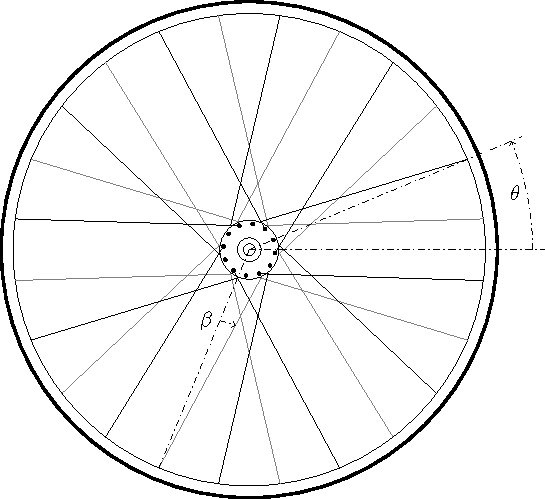
\includegraphics[width=0.375\textwidth]{geom}
    }
    \caption{Wheel geometry. (a)  Rim cross section.  The lateral direction is defined to point toward the non-drive side of the wheel.  The radial direction points outwards from the hub.  The spoke angles $\alpha_{{nd}}$ and $\alpha_{{d}}$ provide lateral stiffness to the wheel. (b) Side view of a wheel. The rim angle, $\theta$, is referenced to the valve stem.  The angle, $\beta$, results from the wheel spoke pattern,  A purely radially spoked wheel has $\beta = 0$.}
    \label{fig:geom}
    \end{figure}

\section{Apparatus}
To develop the model a symmetric (i.e., tensioned equally on both sides), I built a front wheel using a Stans ZTR Alpha rim, a White Industries MI5 hub, and 32 DT Swiss Competition spokes in a so-called `three-cross' tangential spoke pattern.  I performed all adjustments on a Centrimaster Comfort wheel truing stand (Fig \ref{fig:apparatus}).  This stand has radial and lateral mechanical dial gauges to measure the rim displacements with 0.1 mm gauge markings. To obtain optimal resolution and minimize data collection time, I used a Canon EOS M digital camera with a 22mm focal length lens to capture images from the dial gauges and then digitized them with  a computer vision algorithm.  I measured the spoke tension using a WheelFanatyk digital tension gauge. This instrument measures the lateral displacement of a spoke under a known spring tension. This displacement is converted to a measured tension based on a lookup table provided by the manufacturer. It has a claimed accuracy of 10\% and the measurements are discretized to 0.01 mm.

\begin{figure}[!t]
\centering
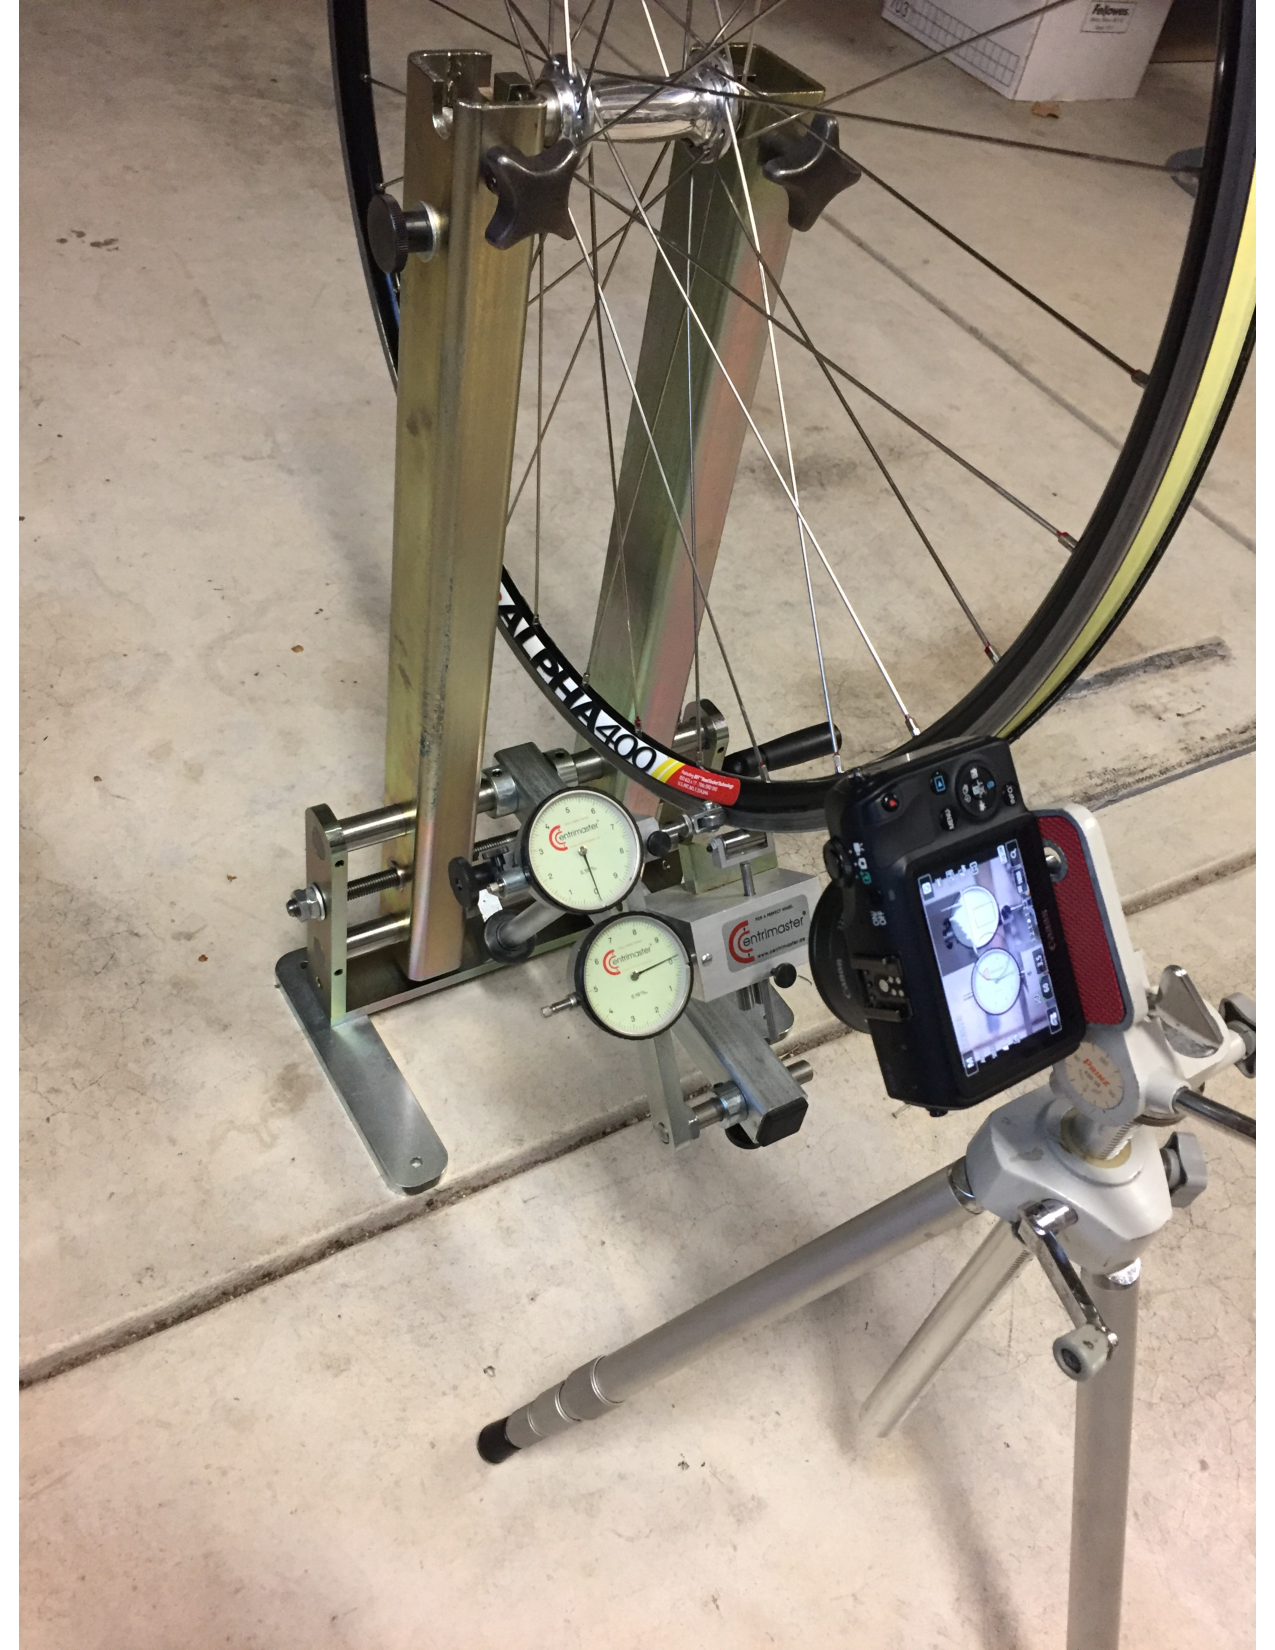
\includegraphics[width=2in]{./imgs/apparat.png}
\caption{Apparatus used to measure lateral and radial displacements.}
\label{fig:apparatus}
\end{figure}

\section{Method}

\subsection{Wheel Model}
The approach taken here is to determine the effect of a constant change in spoke tension on the lateral, radial and tension parameters of a wheel as a function of rim angle.  The resulting curves are referred to as the influence functions of the spoke. To find these influence functions I performed a series of experiments on a subset of the spokes in a given wheel.  For each experiment I loosened a spoke by one complete rotation and took measurements at equal increments along the rim, for the radial and lateral displacements.  I also measured the tension of every spoke. From these data I determined the influence functions and placed them into matrices such that each column represents the influence of a given spoke and each row represents a discrete rim angle.  In other words, if $u_s (\theta), v_s(\theta), \text{ and }t_s(\theta)$ are the lateral and radial influence functions for spoke $s \in [1,2, \cdots , n_s]$, then the influence matrices $\Phi_u, \Phi_v \text{ and } \Phi_t$  for the lateral, radial and tension parameters respectively, at the discrete rim angles $\theta \in [\theta_1,\theta_2,\cdots, \theta_n]$ are given by:

\begin{align*}
    \bf u_s &=  \begin{bmatrix}
        u_s(\theta_1)\\
        u_s(\theta_2)\\
        \vdots\\
        u_s(\theta_n)
        \end{bmatrix}
    \bf v_s = \begin{bmatrix}
        v_s(\theta_1)\\
        v_s(\theta_2)\\
        \vdots\\
        v_s(\theta_n)
    \end{bmatrix}
        \bf t_s = \begin{bmatrix}
        t_s(\theta_1)\\
        t_s(\theta_2)\\
        \vdots\\
        t_s(\theta_n)
    \end{bmatrix}
    \end{align*}
    \begin{align*}
     \Phi_u &= \begin{bmatrix}
     \bf u_1 & \bf u_2& \dots & \bf u_{n_s}
     \end{bmatrix}\\
     \Phi_v &= \begin{bmatrix}
     \bf v_1 & \bf v_2& \dots & \bf v_{n_s}
     \end{bmatrix}\\     
     \Phi_t &= \begin{bmatrix}
     \bf t_1 & \bf t_2& \dots & \bf t_{n_s}
     \end{bmatrix} 
\end{align*}
The influence matrices are the models of the wheel for each parameter.  I combine these matrices into a single matrix $\Phi$:
 \begin{align}
 \Phi = 
     \begin{bmatrix}
         \Phi_u\\
         \Phi_v\\
         \Phi_t
     \end{bmatrix}
     \label{eq:phi}
 \end{align}
Given a vector of tension adjustments (i.e., rotations of the spoke nipples), $\mathbf d$, the prediction of the wheel state after applying the adjustments is given by:
\begin{align}
\mathbf{\hat Y} &= 
     \mathbf{Y_b} + \Phi  \mathbf{d} 
     \label{eq:Y_hat}
 \end{align}
where $\mathbf{\hat Y}$ is the predicted state of the wheel after tensioning and $\mathbf{Y_b}$ is the state of the wheel prior to tensioning. 

To find the optimal vector of spoke tension adjustments, $\mathbf{d}_{ls}$, that results in a measured state (relative to a perfect wheel) at average tension $\bar T$, solve the weighted least squares approximation using a set of measurements $ [ {\bf u,v,T}-\bar T ]$, and the weights $\mu_v \text{ and }\mu_t$:
\begin{align}
    \tilde \Phi &= \begin{bmatrix}
    \Phi_u\\
    \Phi_v \sqrt {\mu_v}\\
    \Phi_t \sqrt {\mu_t}
    \end{bmatrix} \quad
    \bf \tilde Y = \begin{bmatrix}
    \mathbf {u} - u_0 \\
   (\mathbf {v}- v_0)  \sqrt {\mu_v}\\
    ( {\bf  T} - \bar T )  \sqrt {\mu_t}
    \end{bmatrix} 
    \label{eq:y_tilde}
\end{align}
\begin{align}
        {\bf d}_{ls} &= \tilde \Phi^\dagger {\bf \tilde Y}
        \label{eq:dls}
\end{align}
Where $\tilde \Phi^\dagger$ is the pseudo-inverse of $\tilde \Phi$.  Typically $u_0$ and $v_0$ are zero reflecting the fact that the gauge has been set to zero at the desired lateral and radial locations during setup. The weighting factors represent the tradeoff between the lateral, radial, and tension variables and account for the difference in units, the quality of measurements (magnitude and relative noise contribution), as well as the specification for each parameter. In practice, the weighting factors are determined through simulation and validated experimentally. Once ${\bf d}_{ls}$ is found the wheel is trued to its optimal state, ${\bf \hat Y}_{ls}$ by applying $\mathbf{d}_{adj} = -{\bf d}_{ls}$ to the wheel:
\begin{align}
\mathbf{\hat Y}_{ls} &= \mathbf{Y_b} + \Phi  \mathbf{d} _{adj}
\label{eq:Yls}
\end{align}

\subsection{Tension Targeting}
In theory adjusting a wheel to an arbitrary average tension is accomplished by setting $\bar T = T_d$ in (\ref{eq:y_tilde}), where $T_d$ is the desired tension. As will be demonstrated later, however, the tension influence functions are noisy and lack the necessary precision to target tension accurately. Therefore a better method is needed to simultaneously true and tension a wheel to $T_d$.  For this method I exploit the wheel symmetry and make the following observation.  If every spoke of a symmetric wheel is tightened by the same amount then the radial and lateral displacements are unaffected and only the mean tension is changed. It is possible therefore to decouple the average tension change from spoke tension non-uniformity. It should be apparent that this is possible for asymmetric wheels as well, such as a drive wheel or wheel with a disc brake, by compensating for the different spoke angles. 

The approach is as follows.  First calculate ${\bf d}_{ls}$ as in (\ref{eq:dls}) and subtract its mean value.  This is the spoke adjustment vector which will cause a perfectly true wheel to result in the measured wheel state, but without incurring an average tension shift. As before, $\mathbf {d}$ is the vector that transforms the wheel to the trued state:
\begin{align*}
    \mathbf{d} &= -(\mathbf{d}_{ls} - \bar d_{ls})\\
\end{align*}
If the adjustments, $\mathbf {d}$, are applied to the spokes, the lateral, radial and tension variations will be minimized as before, but without changing the average tension.  To determine the necessary constant shift $d_{cm}$ to bring the average tension to $T_d$ calculate the following:
\begin{align*}
    d_{cm} &=  (T_d - \bar T)/c
\end{align*}
Where the proportionality constant, $c$, is the change in mean tension of the wheel when all the spoke nipples are rotated by one revolution. The spoke vector that will optimally true the wheel is:
\begin{align}
    \mathbf{d}_{adj} =\mathbf{d}  + d_{cm} 
\end{align}

\subsection{Optical Digitization}
The method for converting the analog dial gauge readings into digital measurements merits some discussion.  Although a mechatronic implementation of a wheel tensioning machine would likely use digital gauges, it is instructive to demonstrate the effectiveness of optical digitization.  Prior to taking measurements two  images are collected.  The first is a reference image taken with the gauge needles outside the range of expected data range.  The second image is taken with the needles set to zero.  With these two images any subsequent image of a measurement is processed in the following manner.  The measurement image is subtracted from the reference image after appropriate smoothing.  If the images are taken under the same conditions, what remains after subtraction is a ghost image of the needles themselves. A binary threshold is applied to the subtracted image and masked.  Finally, the centroid of the needle tip is determined and an angle from the gauge center to the tip is calculated and compared to the measurement at zero.  The angle is then converted into displacement using the gauge resolution. This process is demonstrated in Fig(\ref{fig:cv_img}).  

\begin{figure}[!t]
    \centering
    \subfloat[]{
        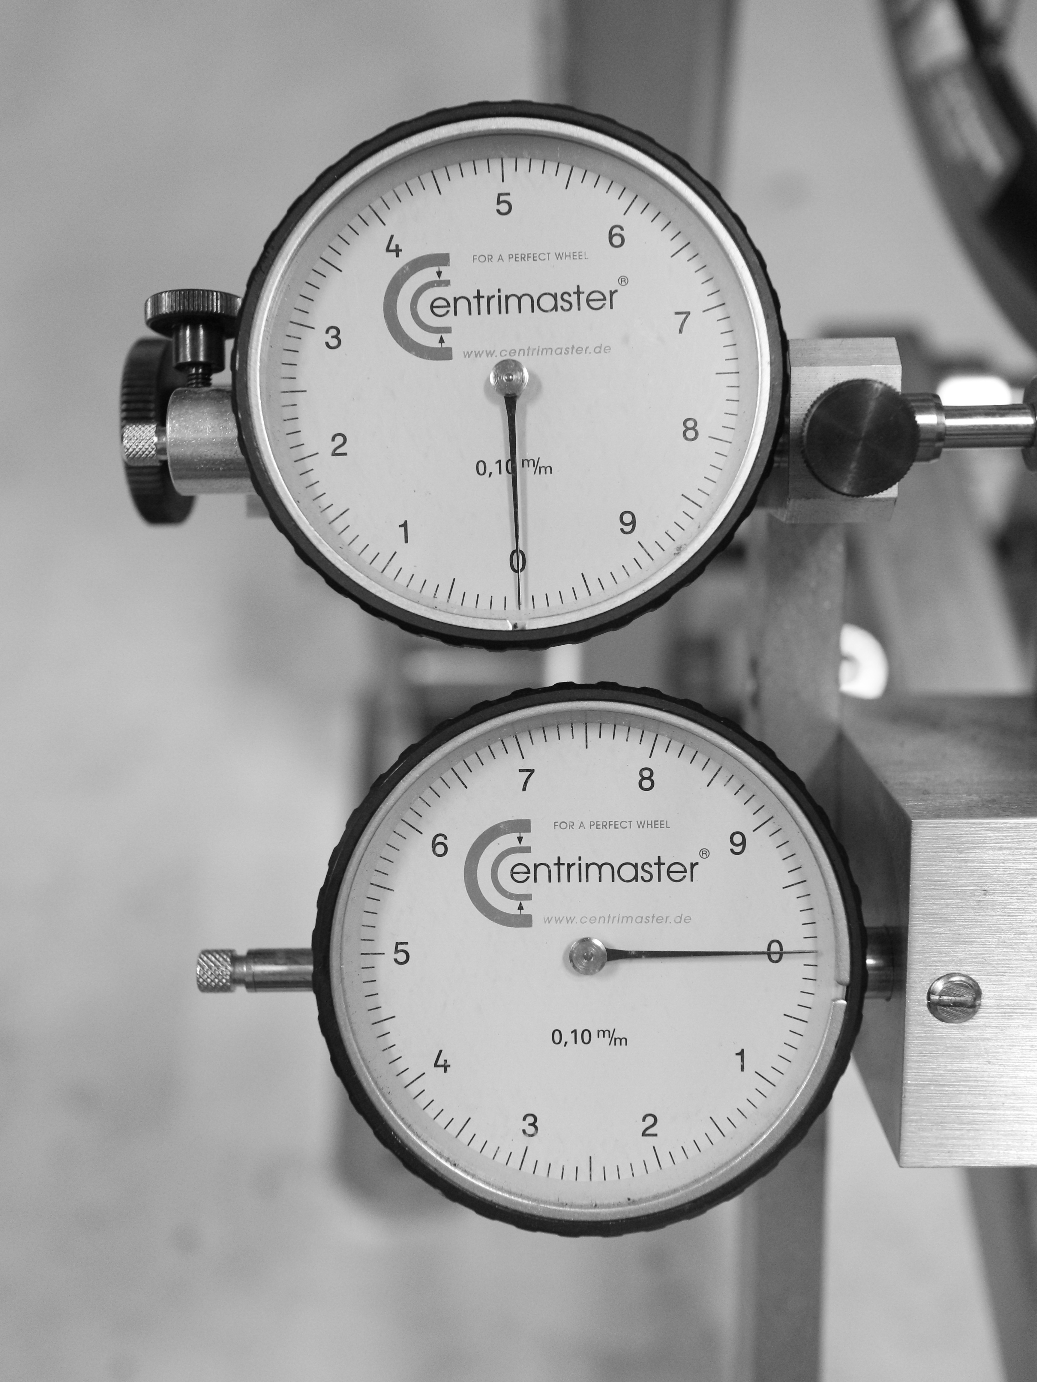
\includegraphics[width=0.2\textwidth]{./imgs/zero}
    }
    \quad
    \subfloat[]{
        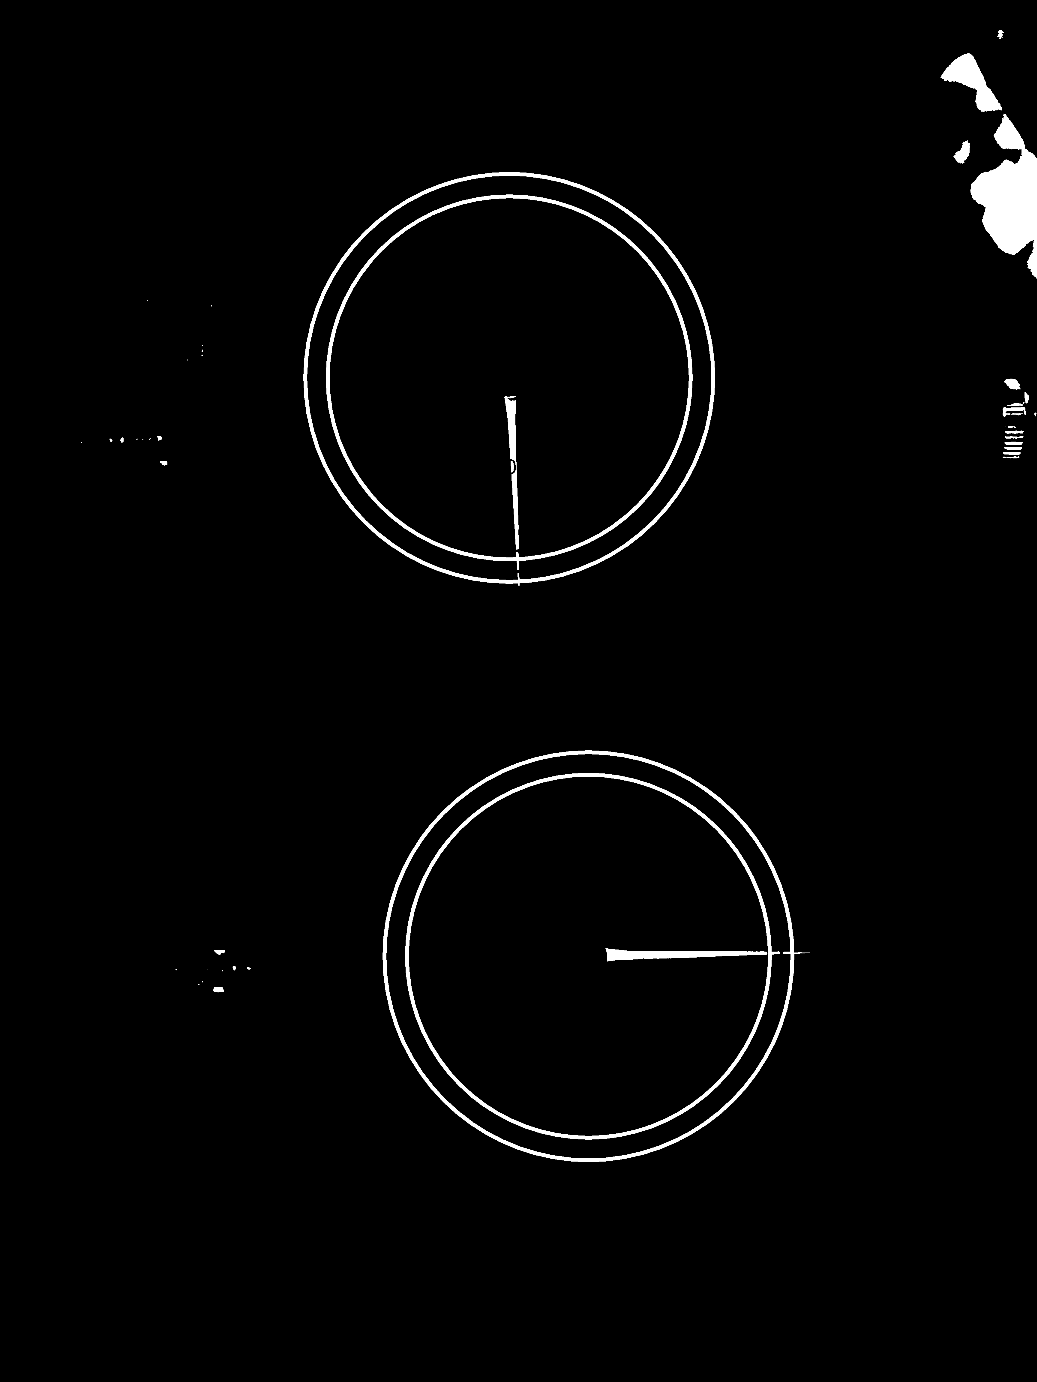
\includegraphics[width=0.2\textwidth]{./imgs/threshold_img}
    }
    \caption{Images used to measure analog dial gauges with computer vision. Image (a) is the measurement image.  Image (b) is generated by subtracting the measurement image from a reference image and applying binary threshold and masking operations (concentric circles). The angle of the needles is measured relative to the gauge center and the converted to a displacement measurement.}
    \label{fig:cv_img}
\end{figure}

\subsection{Wheel Truing Algorithm}
Having determined the optimal spoke adjustments, ${\bf d}_{adj}$, the remaining task is to apply them to the wheel. Although this sounds deceptively simple, there are some difficulties doing this accurately.  The main one is a problem of spoke twist. Spokes are not torsionally stiff and will twist significantly during nipple rotation.  Thus it is difficult to determine precisely how far the spoke nipple has been adjusted based entirely on the rotation angle of the spoke nipple. The servo accuracy or precision may also be inadequate, leading to the accumulation of errors over multiple spoke adjustments. This is particularly true at higher spoke tensions where the friction of the nipple-spoke interface can lead to discrete jumps in nipple rotation. Finally, even if the nipple has been adjusted properly but the spoke is twisted, over time it can untwist which may result in tension loss of the spoke and cause the wheel to go out of true. 

Although the use of high precision servos and clamping the spoke during adjustment can improve the wheel truing process, this paper demonstrates a method that minimizes these sources of variability using lateral feedback during each spoke adjustment. The method begins with the first element of ${\bf d}_{adj}$, the rotation of the first spoke nipple.  Predict the lateral displacement of the rim at the spoke angle of that element using (\ref{eq:Y_hat}).  Adjust the spoke tension until the lateral measurement equals the target displacement. Eliminate spoke twist by measuring the spoke rotation hysteresis during adjustment (also using the lateral gauge feedback) and set the spoke nipple angle midway in the hysteresis regime. Then predict the lateral state at the rim angle of the second spoke using the current state as the new baseline.  Adjust the second spoke tension until the target is reached in the same manner of the first. Continue this process for every element in ${\bf d}_{adj}$.  Fig(\ref{fig:algo}) shows the predicted lateral states of a wheel after each spoke adjustment along with the lateral targets (diamond symbols). These targets were used to true the wheel for the experiment shown in Fig(\ref{fig:exp2}) in the next section. The dashed line represents the lateral state of the wheel prior to tuning, the thin lines show each intermediate state prediction, and the thick line is the prediction of the final state. The algorithm applies each adjustment from the spoke with the smallest angle proceeding sequentially to the spoke at the highest rim angle. In practice some adjustments are too small to perform and can be safely ignored if the wheel state at that spoke is already close to the target within an acceptable tolerance.

\begin{figure}[!t]
\centering
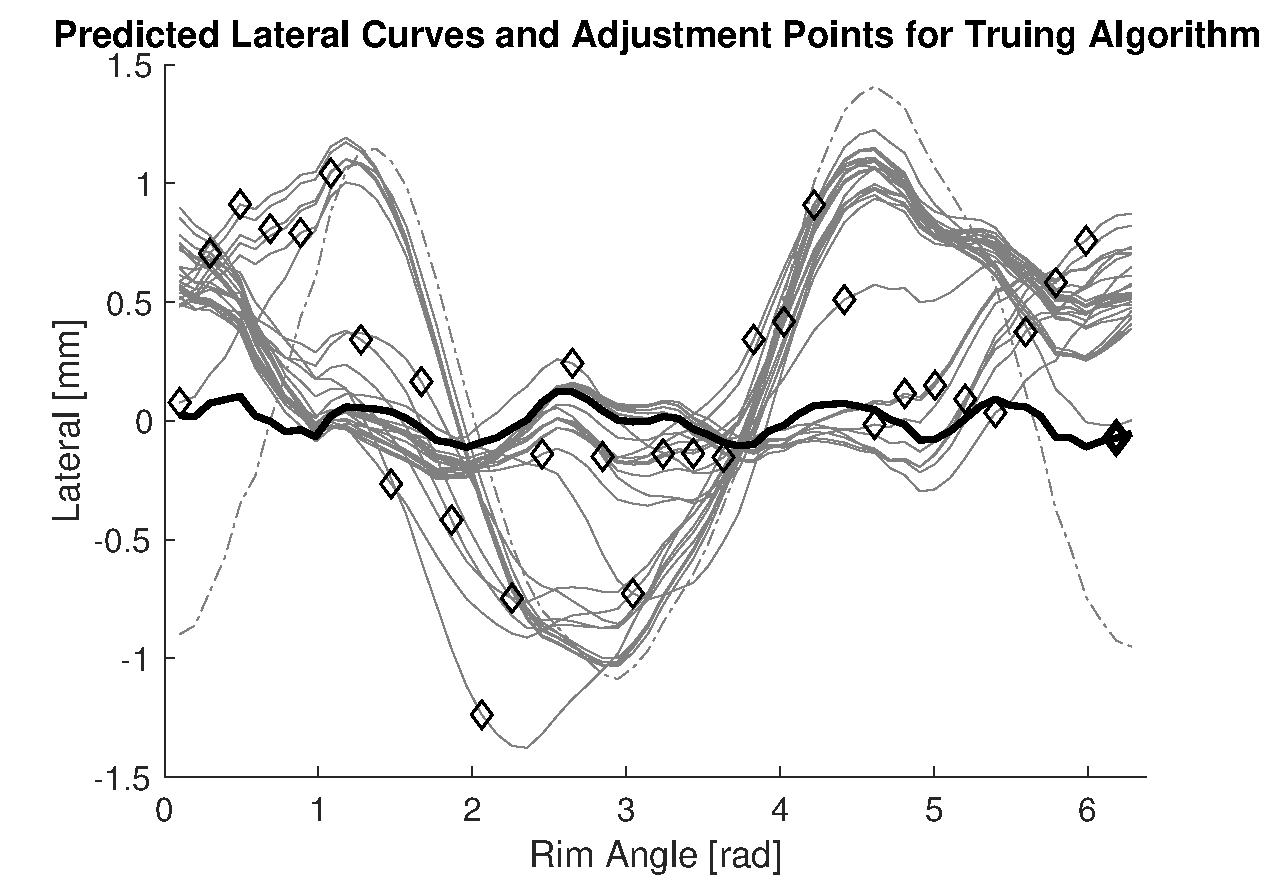
\includegraphics[width=3.5 in]{./figs/algo}
\caption{Example of the truing algorithm. The dashed line is the baseline lateral state.  The thin lines are the predicted states after each spoke adjustment. The spoke tension is adjusted until the lateral measurement equals the diamond target and proceeds from the first spoke (leftmost) to the last.  The thick line is the predicted final state with its truing target. }
\label{fig:algo}
\end{figure}

\section{Results}
\subsection{Optical Digitization of Lateral and Radial Measurements}
To validate the computer vision algorithm described in the previous section, I evaluated the measurement reliability using a series of four images.  I first analyzed their readings manually (through pixel level measurement of the angle of the needles) and then compared against the results returned by the algorithm.  I set both dial gauges to approximately the following settings:  1.0 mm, 0.5 mm, 0.25 mm, and 0.0 mm.  Fig(\ref{fig:cv}) shows the comparison between the two methods.  The estimated effective displacement resolution of the manual measurement method is approximately 0.014 mm.  The computer vision algorithm returned values within $\pm$0.007 mm of the manual measurements. 
\begin{figure}[!t]
\centering
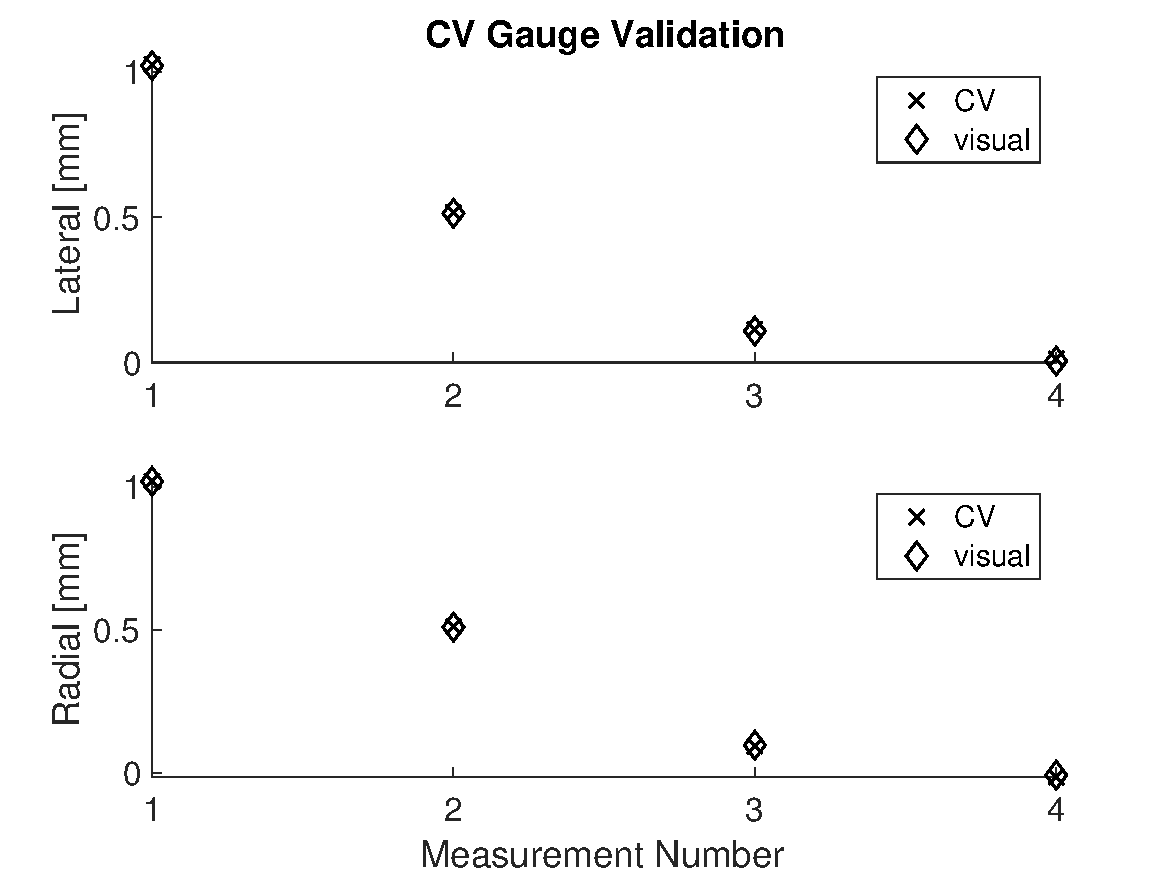
\includegraphics[width=3.25 in]{./figs/CV}
\caption{Validation of the computer vision algorithm developed to interpret analog dial gauge measurements. The results of the two approaches are within the estimate of the resolution of the manual technique.}
\label{fig:cv}
\end{figure}

\subsection{Influence Functions}
I measured Influence functions for every spoke, 32 in total, by loosening the spoke nipple by one complete rotation. For each influence function I measured the lateral and radial displacements at 64 equally spaced locations on the rim starting at the first spoke. To minimize spoke twist in the estimation of the rotation, I marked the spokes and nipples prior to the rotation. A full rotation of the nipple brought the marks back into alignment. I averaged the curves (after normalizing them to the same rim angle) and in the case of the radial displacement, subtracted the mean value. As stated earlier this is due to my assumption that the rim is incompressible in the tangential direction, thus a tension change does not change the average radius.  The subsequent influence functions are shown in Fig(\ref{fig:gclr}).  For each tension influence function I measured the tension of every spoke after loosening the spoke by a full rotation, thus each tension influence function has 32 measurements. This particular spoking geometry results in four distinct tension patterns, depending on whether the spoke is on the drive side of the wheel, or the non-drive side, and whether it is a `leading' spoke or a `trailing' spoke, that is whether its spoke angle, $\beta$, is positive or negative (see Fig(\ref{fig:geom}).  Because this is a symmetric wheel, however, the non-drive side leading spoke influence function is a mirror image of the drive side trailing one.  Similarly, the non-drive side trailing spoke influence function is a mirror image of the drive side leading one. I exploited this symmetry to generate the four tension influence functions in Fig(\ref{fig:gc_ten}), such that each function represents the average of 16 measured curves and is mirrored when necessary.

The lateral and radial influence functions can be used directly and put into the influence matrices.  Alternatively, they can be fit to the Fourier series which is an ideal modeling method for these functions due to their continuous nature and $2\pi$ periodicity.  The Fourier series takes the form:
\begin{align*}
y(\theta) =a_0 + \sum_{n=1}^{N} a_n\cos(n\theta) + b_n\sin(n\theta)
\end{align*}
where $n\theta$ is the spatial frequency of the mode of oscillation and $y(\theta$) is the function to be fitted.  To develop the model of these functions I randomly divided the set of measured influence functions into two sets, a modeling set and a testing set.  I fit the modeling set to the Fourier series to find the coefficients $a_n, b_n$ using least squares.  I determined the highest significant spatial frequency by plotting the sum squared residual error between the modeling and testing sets against the number of fitting coefficients, and therefore spatial frequency. This is plotted in Fig(\ref{fig:Fourier}).  It is evident from this plot that the residual error for the lateral influence function is reduced in the testing data set up to a spatial frequency, $N_{lat} = 6$ (i.e., 13 fitting coefficients) and up to $N_{rad} = 13$ (27 fitting coefficients) for the radial influence function. Because the mean influence functions of Fig(\ref{fig:gclr}) exhibit little noise, I used them for the model in this work.  If there were fewer measured functions, however, using the modeled approach would be more appropriate. 

\begin{figure}[!t]
\centering
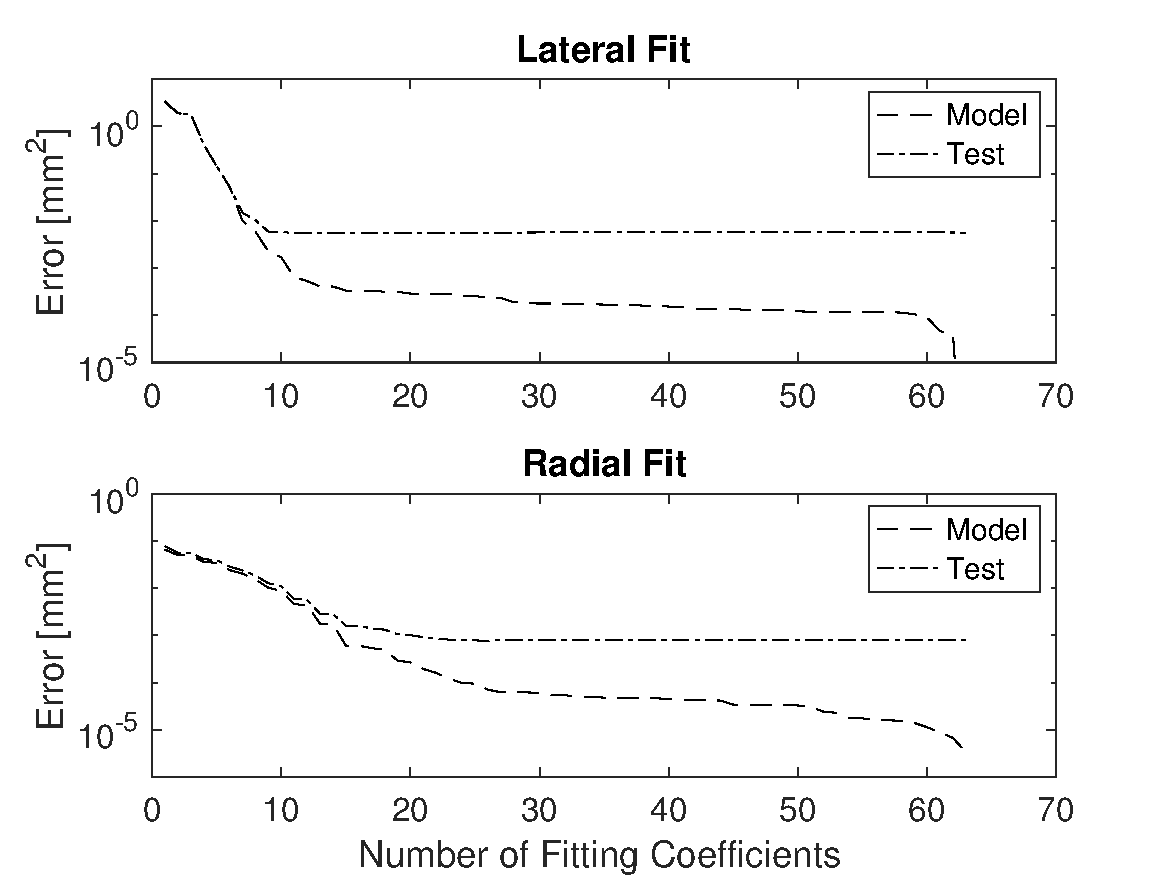
\includegraphics[width=3.25 in]{./figs/Fourier}
\caption{Residual error vs fitting coefficient number for the lateral and radial influence functions when fit to a Fourier series.  I used the residual of the testing set to determine the highest spatial frequency to be used for the model. Although difficult to discern due to the log scale, the residual error increases in the lateral testing set for fitting coefficients beyond 13, corresponding to $N_{lat}=6$.  Similarly I determined the highest mode of oscillation for the radial influence function to be $N_{rad} = 13$.}
\label{fig:Fourier}
\end{figure}

The tension measurements are inherently discrete so fitting them to a Fourier series, while feasible, has no meaning. There are analytical models available for them (see \cite{ModeMatrix} for an open source example), however, they require characterization of the rim that is not practical \emph{in-situ}.  Therefore, for this work I used only the averaged data for the tension influence matrix.  

\begin{figure}[!t]
\centering
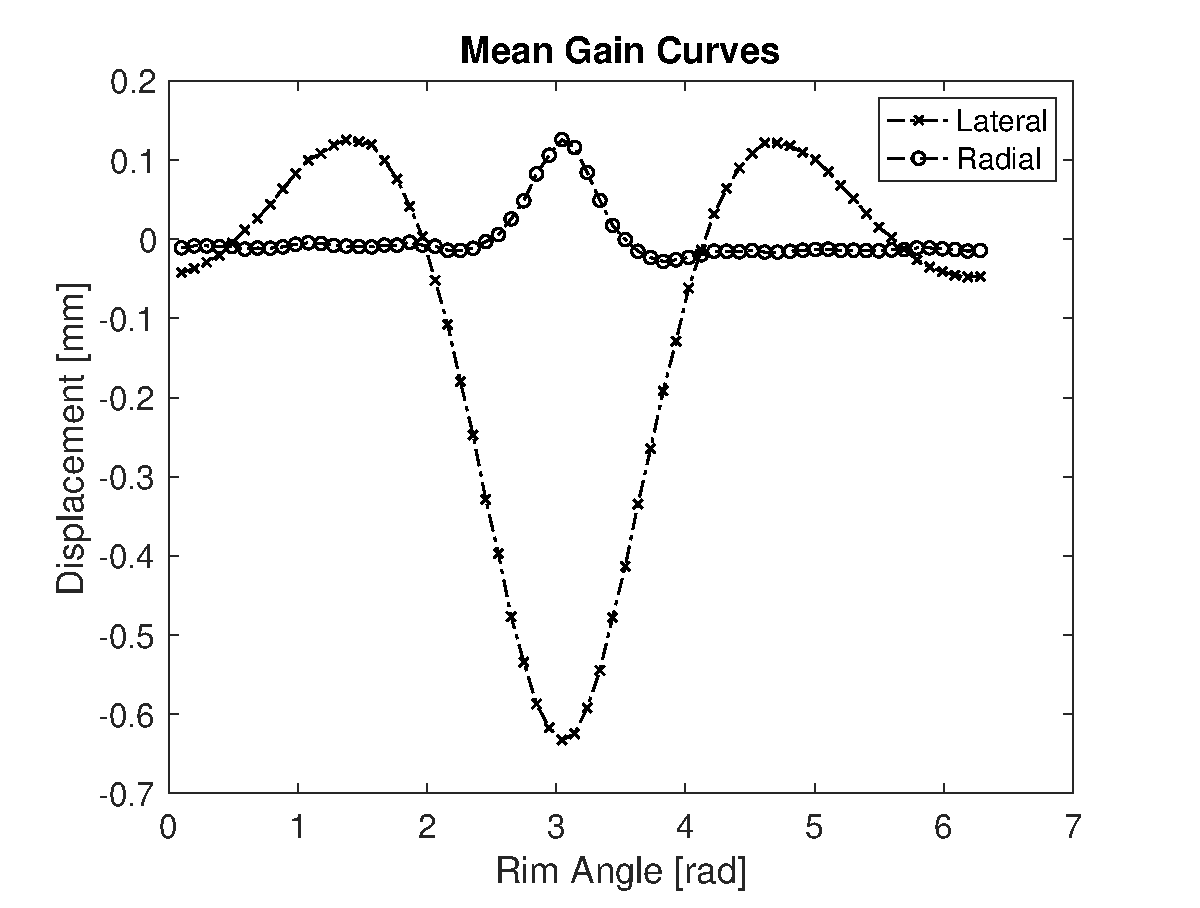
\includegraphics[width=3.25 in]{./figs/gc_lat_rad}
\caption{The mean influence functions for the lateral and radial parameters.  These functions are the average of 32 measured curves after normalizing them to the angle of the 16th spoke.}
\label{fig:gclr}
\end{figure}

\begin{figure}[!t]
\centering
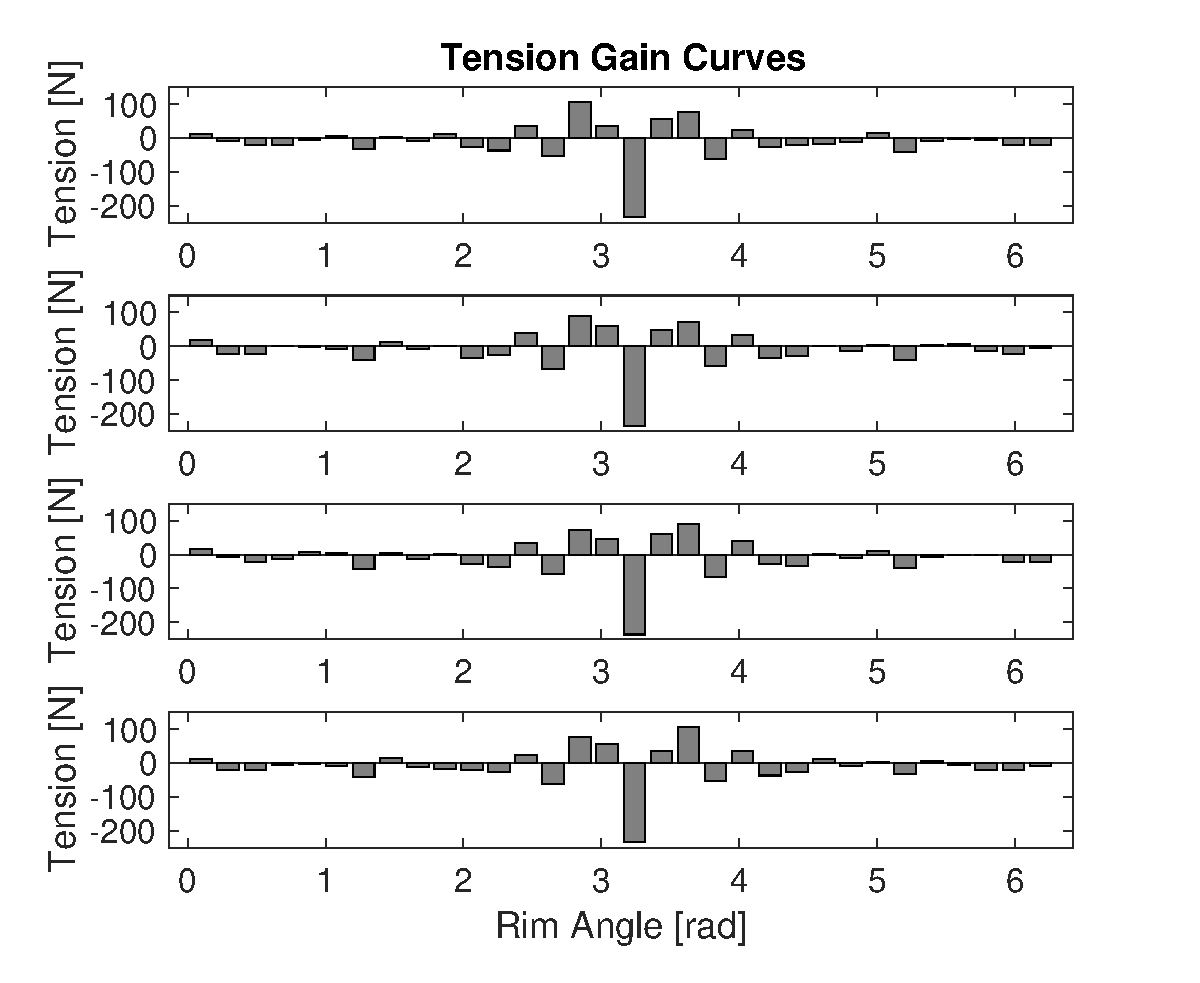
\includegraphics[width=3.25 in]{./figs/gc_ten}
\caption{The mean influence functions for spoke tension. From top to bottom: (a) Non-drive side leading. (b) Drive-side leading. (c) Non-drive side trailing. (d) Drive side trailing.  Note that (a) and (d) are mirror images, as are (b) and (c).}
\label{fig:gc_ten}
\end{figure}

Regardless of whether the model or the data are used in the influence functions, however, it should be clear that the influence matrices composed of those functions will be less than full rank.  This can be understood because the highest order spatial frequency that appears in the model is 13, corresponding to 27 basis vectors associated with the Fourier coefficients. This satisfies an intuitive understanding of the wheel structure particularly the fact that there are two degrees of freedom that are not taken into account in the wheel model, namely the tangential stiffness and the torsional stiffness of the rim, and that the mean tension of the wheel can be changed without affecting any of the displacement parameters. This can be independently verified by performing a singular value decomposition of the influence matrices composed of solely averaged data for the influence functions, shown in Fig(\ref{fig:svd}). It is evident that without the inclusion of the tension influence matrix the model of the wheel is underdetermined.  

\begin{figure}[!t]
\centering
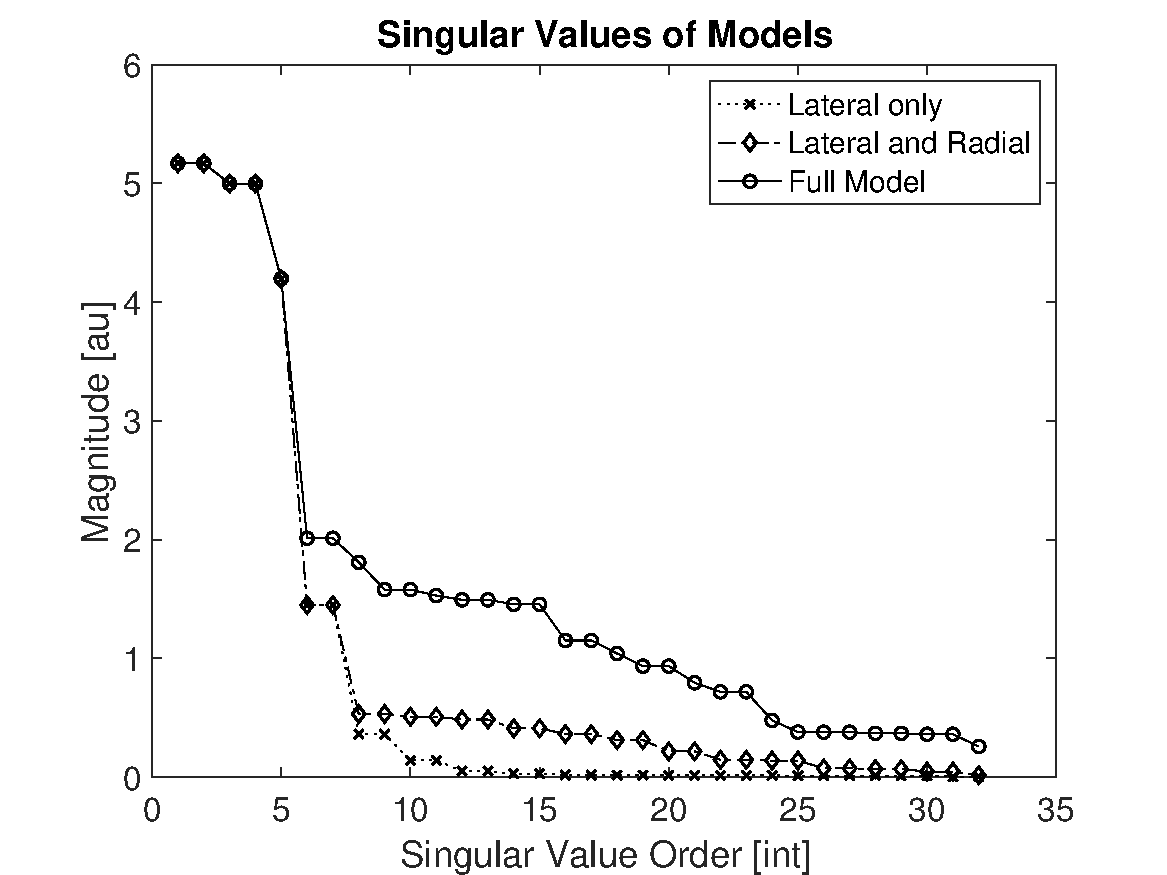
\includegraphics[width=3.25 in]{./figs/svd}
\caption{The singular values associated with the singular value decomposition of the following influence matrices: lateral, the concatenation of the lateral and the radial, and the full model.}
\label{fig:svd}
\end{figure}

\subsection{Simulation}
With the influence matrices developed as in (\ref{eq:phi}) the state of the wheel can be predicted for a given spoke tensioning vector. To predict $d_{ls}$ however, the weighting parameters $\mu_v$ and $\mu_t$ need to be determined through simulation. Additionally, given the relatively noisy and coarsely discretized influence functions discuss in the previous section, I simulated an alternative approach for finding $d_{ls}$ using a regularization technique.  

Regularization is the process of concatenating the identity matrix in place of the tension influence matrix in $\tilde \Phi$ and the zero vector in $\bf \tilde Y$ in place of the tension measurements:
\begin{align}
    \tilde \Phi &= \begin{bmatrix}
    \Phi_u\\
    \Phi_v \sqrt {\mu_v}\\
   I \mu_I
    \end{bmatrix} \quad
    \bf \tilde Y = \begin{bmatrix}
    \mathbf {u} - u_0 \\
   (\mathbf {v}- v_0)  \sqrt {\mu_v}\\
   \bf 0
    \end{bmatrix} 
    \label{eq:y_tilde2}
\end{align}
where $\mu_I$ is a weighting factor for the identity matrix. Regularization has the effect of minimizing $||\bf d_{ls}||$ when solved for as in (\ref{eq:dls}). The hypothesis for this technique is that the value of $||\bf d_{ls}||$ that is the smallest is the one that also will minimize tension variations in the solution. 

I performed simulations for both the regularized influence matrices, as well as the full model in order to determine the weighting factors. For each simulation I generated a random vector of spoke adjustments and calculated a wheel state prediction using (\ref{eq:Y_hat}). To this wheel state I added white noise to simulate the uncertainty of the measurement.  I determined the noise distributions from the measured profiles generated during the influence function development.  I developed the initial weighting factors based on a comparison of the magnitude of the changes induced by a unit disturbance of the three parameters, normalized to the maximum lateral displacement. I then computed the weighted least squares estimation of the random spoke vector $\bf d_{ls}$ using these weighting factors and  predicted final state of the wheel using (\ref{eq:Yls}). I modified the weighting factors until the predicted performance error of each algorithm was minimized relative to actual spoke vector used to generate the given wheel state. Fig(\ref{fig:simd}) shows the result of one such simulation. In general the full model outperformed the regularized model by at least 2$\times$. The predicted spoke vector for the full model is generally agrees to an rms of $\leq$ 0.1 revolutions.  After extensive simulation I found acceptable weighting factors of: $\mu_v = 0.5$, $ \mu_t =10^{-5}$.

\begin{figure}[!t]
\centering
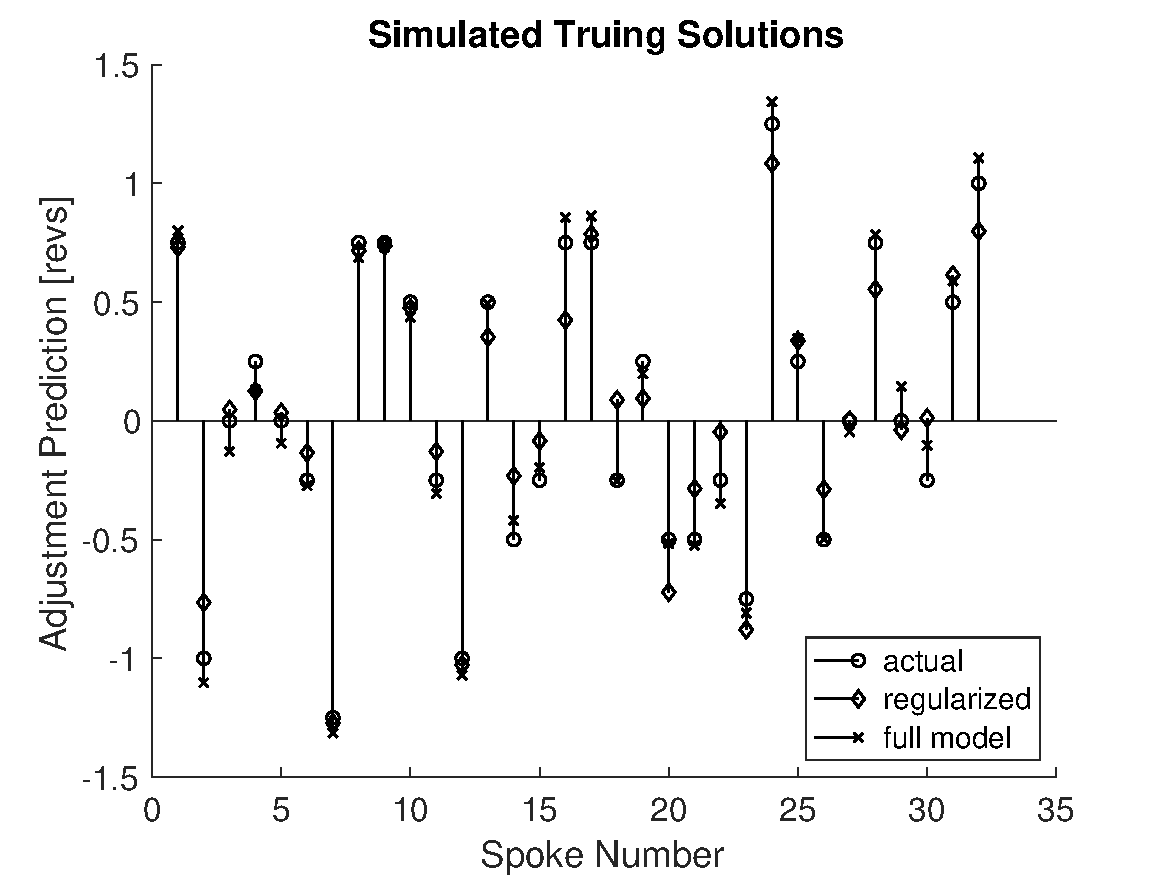
\includegraphics[width=3.25 in]{./figs/simd2}
\caption{Example of the simulation process used to determine the weighting factors for the multi-objective least squares approximation. The circles represent the actual spoke adjustments for a given simulation and the other symbols represent the approximations from two different approaches: a regularized model and the full model.  On average, regularization resulted in estimation errors 2$\times$ worse than when using the full model.}
\label{fig:simd}
\end{figure}

\subsection{Model Validation}
The model is separated into two parts, spoke adjustments which affect the variations in the wheel parameters while preserving the mean tension, and adjustments which affect the mean tension of the wheel but do not affect parameter uniformity.  I found the latter part of the model by determining the coefficient, $c$, between the average of the spoke adjustment vector and the average tension change of the wheel.  Fig(\ref{fig:c}) demonstrates the results of seven experiments. A linear fit to these data finds $c=-$473 N/rev. In practice, this constant could be derived from a single experiment where every spoke is adjusted by one revolution. 

 \begin{figure}[!t]
\centering
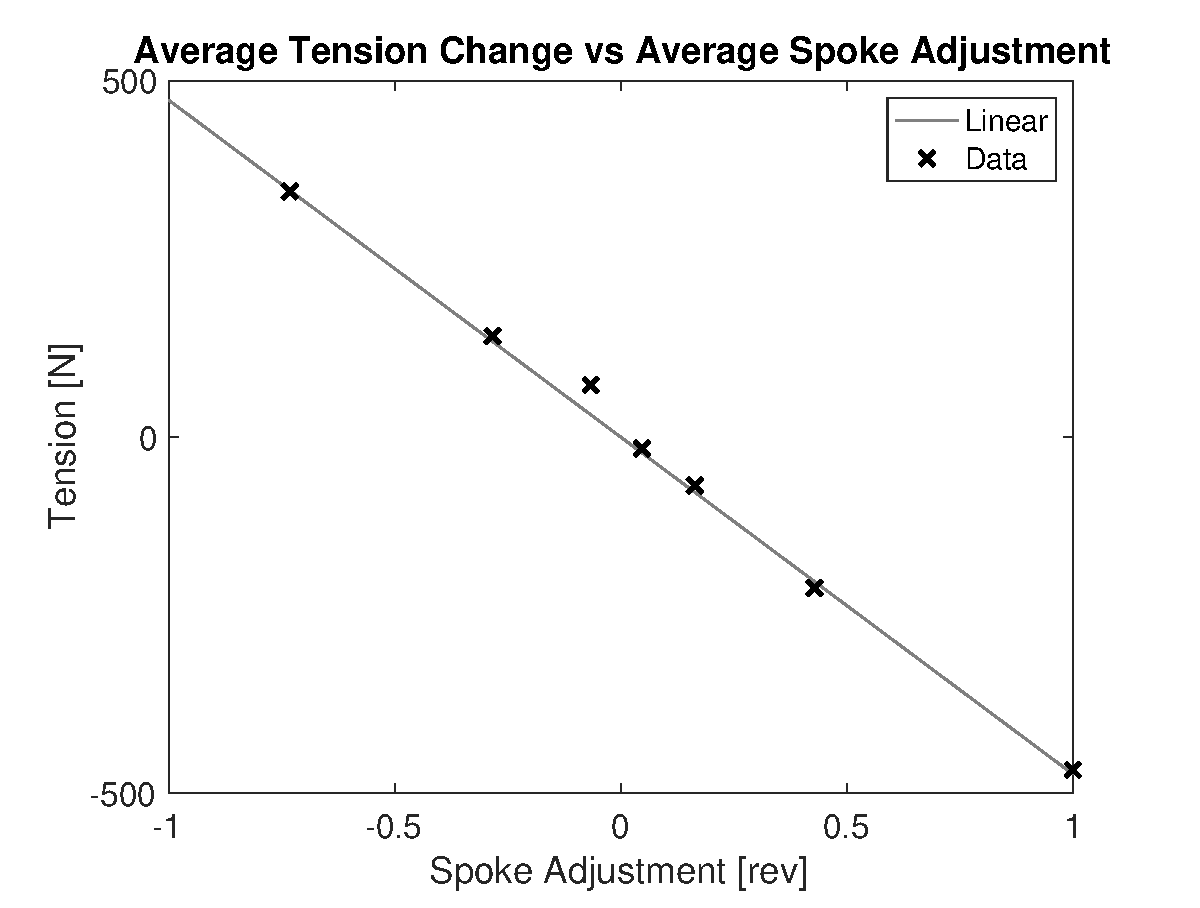
\includegraphics[width=3.25 in]{./figs/c}
\caption{The average tension change of a wheel due to the average spoke adjustment. A linear fit to the data finds $c=-473 N/rev$.}
\label{fig:c}
\end{figure}

To validate the model performance for spoke adjustment vectors that affect the variations in the wheel parameters while preserving the mean tension, I performed a different experiment.  In this case I applied a random spoke adjustments vector to the (manually trued) test wheel and compared the resulting measured wheel parameters to the model predictions. Fig(\ref{fig:exp1}) shows the result of this experiment and Fig(\ref{fig:exp1_err}) shows the residual error of model after the adjustment. The rms model error of the lateral, radial and tension parameters are 0.123mm, 0.049mm, and 33N, respectively.  The model fits the data well considering the tolerance of the lateral adjustment which is estimated to be approximately 0.1mm.

Finally, to demonstrate the need for separating the model into two parts is demonstrated in Fig(\ref{fig:exp_cnst_shift}).  For this experiment, I targeted a well-trued wheel (tensioned to 780N) to a new tension target of 1000N using (\ref{eq:y_tilde}).  I applied the resulting spoke adjustment vector to the wheel.  Table(\ref{tbl:const_shift}) summarizes the results of this experiment. Although the wheel is still true the tension exceeds the target by 126N and the tension non-uniformity is 1.5$\times$ worse than the initial state in percentage terms (4.2\% vs 6.8\%). The reason for the failure of the model in this regime appears to be related to the tension influence functions themselves and is likely due to the relatively large discretization errors of the tension measurement (nearly 4\% at 1000N).  Without finer resolution these discretization errors accumulate when a constant value is added to the spoke adjustment solution.  Although better instrumentation and rigorous analysis of the influence functions would likely improve the model, calculating the average tension change separately is a superior solution as the average tension change is easily measured independently. 

\begin{figure}[!t]
\centering
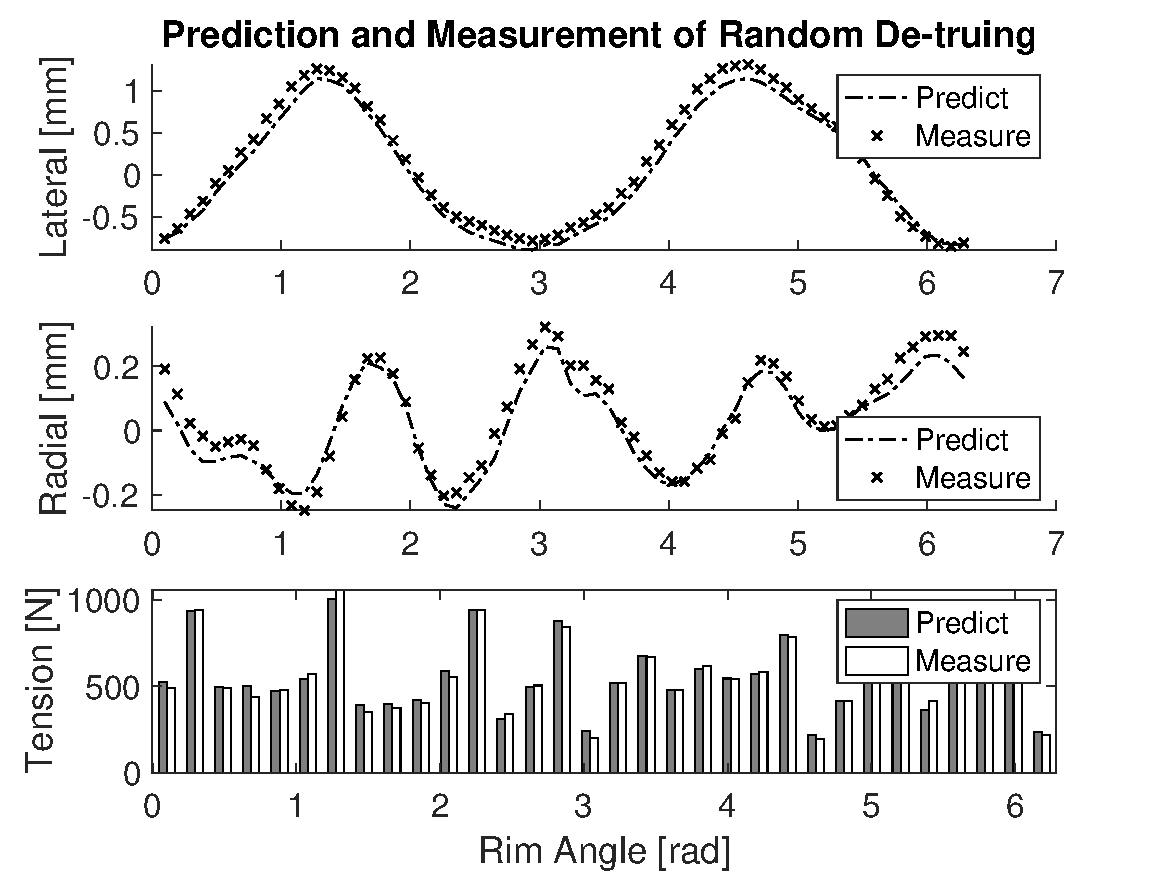
\includegraphics[width=3.25 in]{./figs/exp1} %this is the detruing experiment
\caption{The actual and predicted lateral, radial, and tension values for the random de-truing experiment.}
\label{fig:exp1}
\end{figure}

\begin{figure}[!t]
\centering
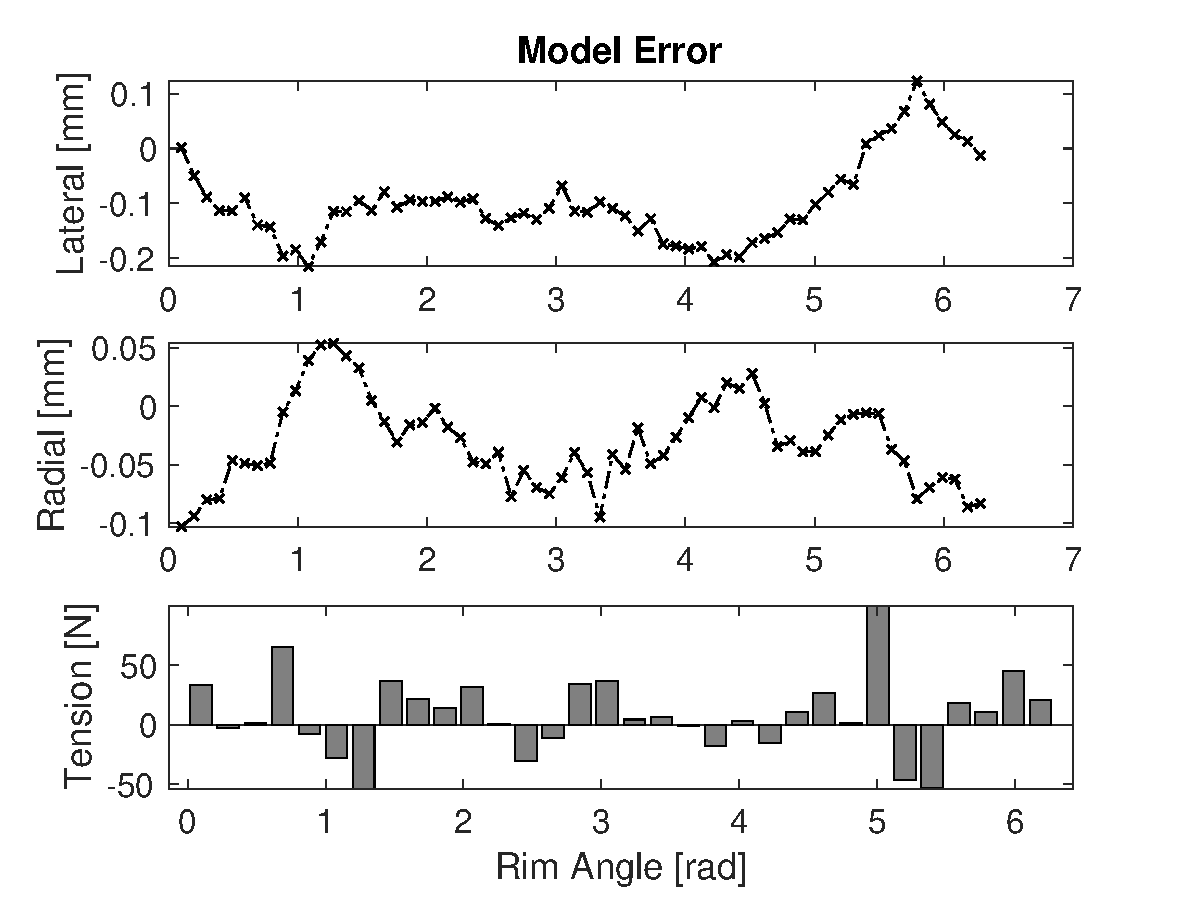
\includegraphics[width=3.25 in]{./figs/exp1_err} %error in the detruing experiment
\caption{The model error relative to the measurements for the random de-truing experiment.  The rms errors are found to be 0.123 mm (lateral), 0.049 mm (radial), and 33 N (tension).}
\label{fig:exp1_err}
\end{figure}

\begin{figure}[!t]
\centering
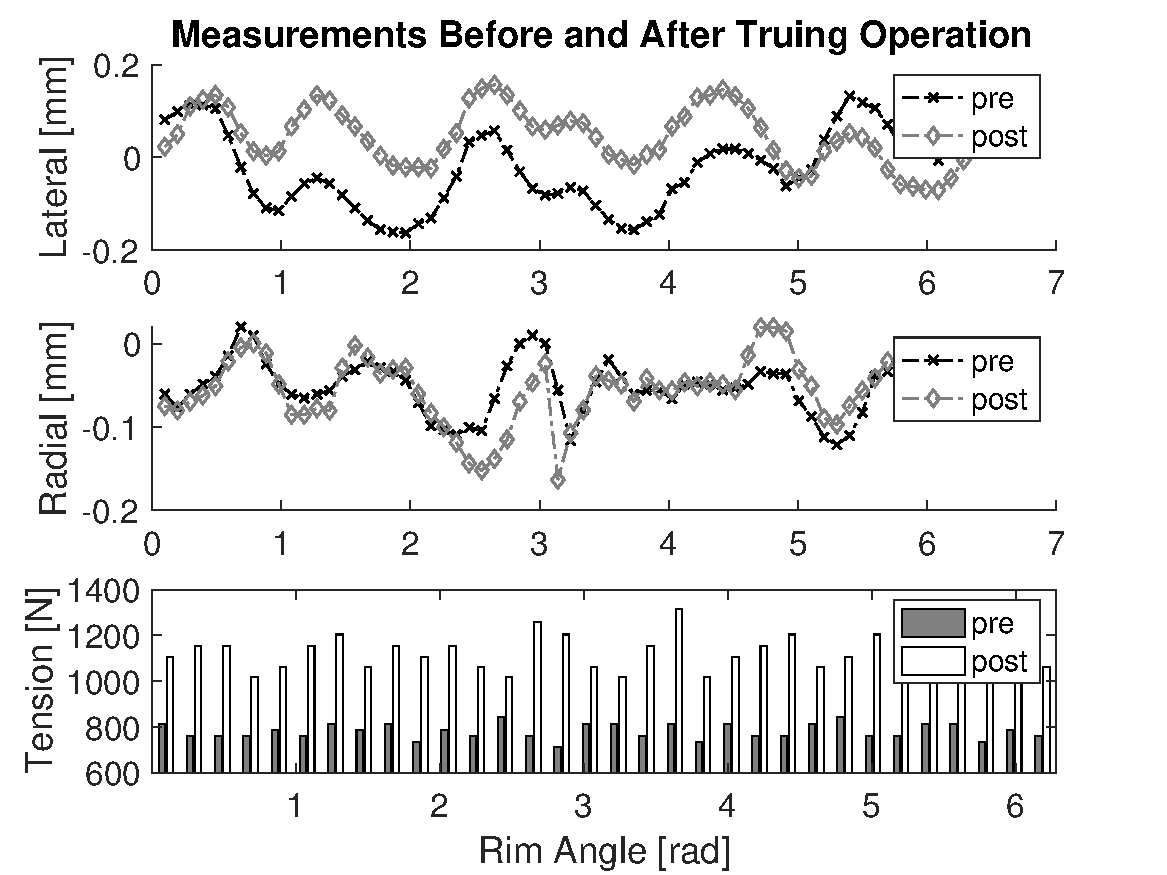
\includegraphics[width=3.25 in]{./figs/exp_cnst_shift} % Change tension using original model
\caption{Changing the tension of true wheel using the model described in (\ref{eq:y_tilde}).  Although the wheel remains true the tension target of 1000N is significantly exceeded and has more variability. }
\label{fig:exp_cnst_shift}
\end{figure}

\begin{table}[!t]
\caption{Results of Changing Tension}
\label{tbl:const_shift}
\centering
\begin{tabular}{| l | c | c |}
    \hline
    Parameter & Inital ($\mu \pm \sigma$) & Final ($\mu \pm \sigma$)\\ \hline
    Lateral [mm] & $-0.029\pm0.083$ &$0.045\pm 0.063$ \\ \hline 
    Radial [mm] &$-0.052\pm0.032$& $-0.056\pm0.039$ \\ \hline 
    Tension [N] &$781\pm33$& $1126\pm76$ \\ \hline 
\end{tabular}
\end{table}

\subsection{Wheel Truing Validation}
To validate the complete model and truing algorithm I applied the truing algorithm to a randomly de-trued wheel with a target tension of 1000 N. The initial wheel state was not only substantially out of true, with lateral variations of more than $\pm1$mm, but also at a very low average tension of 556N with tension variation of $\pm$500N.  Despite  this, the algorithm trued the wheel to its target tension within 9N and the improved resulting non-uniformity for all parameters by nearly 500\% in a single iteration. Fig(\ref{fig:exp2}) shows the wheel state before and after the truing operation and Table(\ref{tbl:exp2}) summarizes the measurements. The maximum variations are 0.17 mm above the mean (lateral), 0.07 mm above the mean (radial), and 104 N below the mean (tension). 

Finally, I iterated the truing algorithm to see whether the wheel truing performance improved.  The results are shown in Table(\ref{tbl:exp3}). The non-uniformity improved modestly for every parameter and the mean tension was still within measurement error of the targeted value. 

\begin{table}[!t]
\caption{Truing algorithm results}
\label{tbl:exp2}
\centering
\begin{tabular}{| l | c | c |}
    \hline
    Parameter & Inital ($\mu \pm \sigma$) & Final ($\mu \pm \sigma$)\\ \hline
    Lateral [mm] & $0.160\pm0.736$ &$-0.037\pm 0.107$ \\ \hline 
    Radial [mm] &$0.050\pm0.158$& $-0.046\pm0.047$ \\ \hline 
    Tension [N] &$556\pm211$& $1009\pm45$ \\ \hline
\end{tabular}
\end{table}

\begin{figure}[!t]
\centering
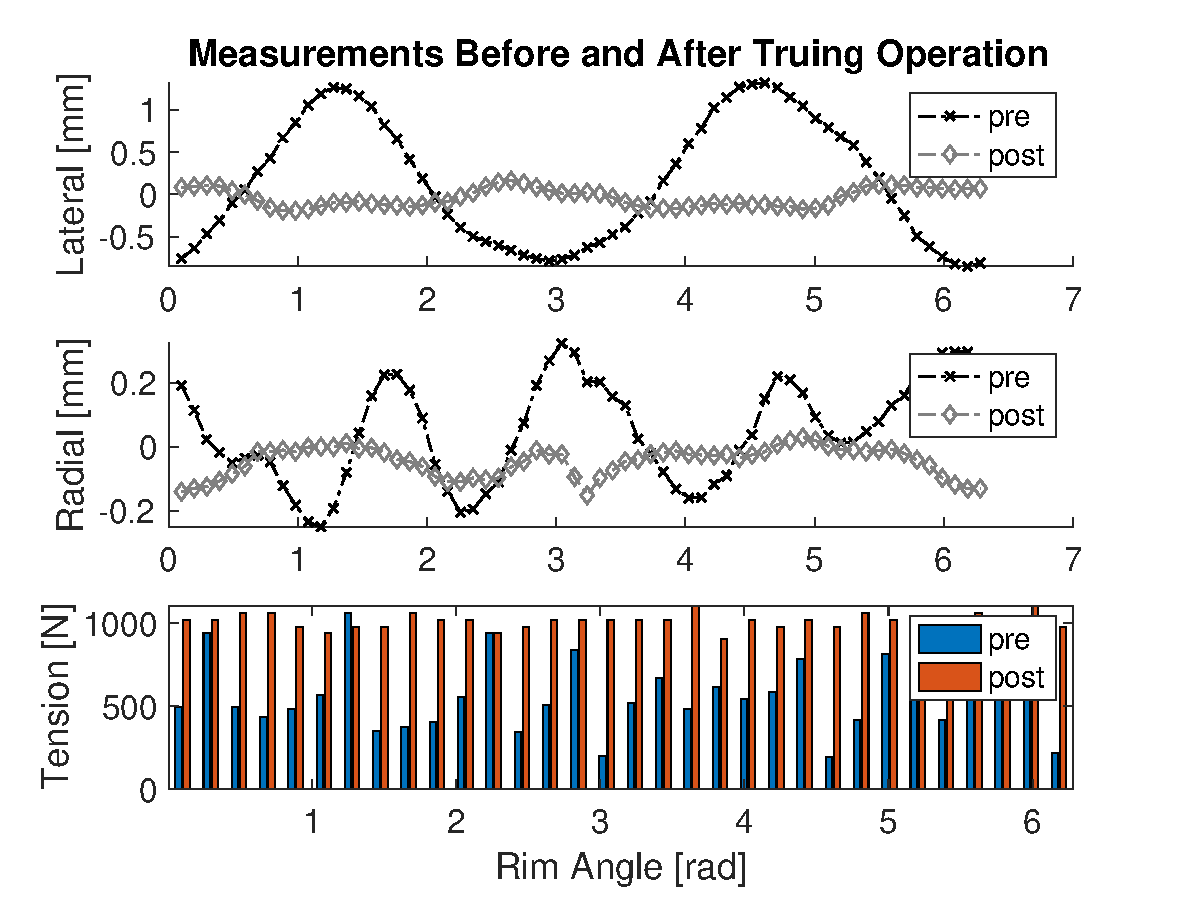
\includegraphics[width=3.25 in]{./figs/exp2}
\caption{The state of the wheel is shown before and after the truing operation. The results are summarized in Table(\ref{tbl:exp2}).}
\label{fig:exp2}
\end{figure}

\begin{table}[!t]
\caption{Second iteration of truing}
\label{tbl:exp3}
\centering
\begin{tabular}{| l | c | c |}
    \hline
    Parameter & Inital ($\mu \pm \sigma$) & Final ($\mu \pm \sigma$)\\ \hline
    Lateral [mm] & $-0.037\pm0.107$ &$0.028\pm 0.073$ \\ \hline 
    Radial [mm] &$-0.046\pm0.047$& $-0.031\pm0.034$ \\ \hline 
    Tension [N] &$1009\pm45$& $989\pm39$ \\ \hline 
\end{tabular}
\end{table}

% needed in second column of first page if using \IEEEpubid
%\IEEEpubidadjcol




% An example of a floating figure using the graphicx package.
% Note that \label must occur AFTER (or within) \caption.
% For figures, \caption should occur after the \includegraphics.
% Note that IEEEtran v1.7 and later has special internal code that
% is designed to preserve the operation of \label within \caption
% even when the captionsoff option is in effect. However, because
% of issues like this, it may be the safest practice to put all your
% \label just after \caption rather than within \caption{}.
%
% Reminder: the "draftcls" or "draftclsnofoot", not "draft", class
% option should be used if it is desired that the figures are to be
% displayed while in draft mode.
%
%\begin{figure}[!t]
%\centering
%\includegraphics[width=2.5in]{myfigure}
% where an .eps filename suffix will be assumed under latex, 
% and a .pdf suffix will be assumed for pdflatex; or what has been declared
% via \DeclareGraphicsExtensions.
%\caption{Simulation results for the network.}
%\label{fig_sim}
%\end{figure}

% Note that the IEEE typically puts floats only at the top, even when this
% results in a large percentage of a column being occupied by floats.


% An example of a double column floating figure using two subfigures.
% (The subfig.sty package must be loaded for this to work.)
% The subfigure \label commands are set within each subfloat command,
% and the \label for the overall figure must come after \caption.
% \hfil is used as a separator to get equal spacing.
% Watch out that the combined width of all the subfigures on a 
% line do not exceed the text width or a line break will occur.
%
%\begin{figure*}[!t]
%\centering
%\subfloat[Case I]{\includegraphics[width=2.5in]{box}%
%\label{fig_first_case}}
%\hfil
%\subfloat[Case II]{\includegraphics[width=2.5in]{box}%
%\label{fig_second_case}}
%\caption{Simulation results for the network.}
%\label{fig_sim}
%\end{figure*}
%
% Note that often IEEE papers with subfigures do not employ subfigure
% captions (using the optional argument to \subfloat[]), but instead will
% reference/describe all of them (a), (b), etc., within the main caption.
% Be aware that for subfig.sty to generate the (a), (b), etc., subfigure
% labels, the optional argument to \subfloat must be present. If a
% subcaption is not desired, just leave its contents blank,
% e.g., \subfloat[].


% An example of a floating table. Note that, for IEEE style tables, the
% \caption command should come BEFORE the table and, given that table
% captions serve much like titles, are usually capitalized except for words
% such as a, an, and, as, at, but, by, for, in, nor, of, on, or, the, to
% and up, which are usually not capitalized unless they are the first or
% last word of the caption. Table text will default to \footnotesize as
% the IEEE normally uses this smaller font for tables.
% The \label must come after \caption as always.
%
%\begin{table}[!t]
%% increase table row spacing, adjust to taste
%\renewcommand{\arraystretch}{1.3}
% if using array.sty, it might be a good idea to tweak the value of
% \extrarowheight as needed to properly center the text within the cells
%\caption{An Example of a Table}
%\label{table_example}
%\centering
%% Some packages, such as MDW tools, offer better commands for making tables
%% than the plain LaTeX2e tabular which is used here.
%\begin{tabular}{|c||c|}
%\hline
%One & Two\\
%\hline
%Three & Four\\
%\hline
%\end{tabular}
%\end{table}


% Note that the IEEE does not put floats in the very first column
% - or typically anywhere on the first page for that matter. Also,
% in-text middle ("here") positioning is typically not used, but it
% is allowed and encouraged for Computer Society conferences (but
% not Computer Society journals). Most IEEE journals/conferences use
% top floats exclusively. 
% Note that, LaTeX2e, unlike IEEE journals/conferences, places
% footnotes above bottom floats. This can be corrected via the
% \fnbelowfloat command of the stfloats package.

\section{Conclusion}
In this work I have successfully demonstrated a linear wheel model developed empirically using a system identification methodology. This modeling technique is easily incorporated into existing robotic wheel manufacturing machines provided they have measurement ability for lateral and radial rim displacements as well as spoke tension measurements. I find that the spoke tension measurements, even if poor quality, are required in order to minimize spoke tension variation in the completed wheel.  The weighting factors used to calculate the optimum truing solution can be adjusted to account for the desired tolerance in the solution or for noisy data making this solution ideal for a manufacturing context. Once a characteristic wheel has been modeled this model can be used to efficiently tension and true subsequent wheels of the same design.

To apply the model to true wheels I developed a truing algorithm that minimizes adjustment errors using a prediction of intermediate wheel states after adjustment of each spoke and lateral measurement feedback. This algorithm trues a wheel in a single iteration even to a significantly different tension than the initial state. The truing algorithm minimizes spoke twist by detecting the hysteresis in the spoke nipple rotation and adjusting the nipple to the approximate midpoint of the hysteresis region once the lateral target is reached. Elimination of spoke twist prevents the wheel from going out of true over time and allows for accurate tension adjustments independent of the actual rotation angle of the nipple rotation mechanism. An important consequence of this approach is that the characterization of the influence functions doesn't rely on an absolute perturbation of the wheel state because the feedback compensates for this effect during truing and because the model is linear.

The main limitation to the model is the inaccuracy and perhaps more importantly the coarse discretization of the tension measurements.  As a consequence, the tension parameter is weighted relatively less than the radial and lateral parameters.  The resulting wheel state after a truing operation reflects this weighting and therefore the tension errors approach 10\%. The main limitation to the truing algorithm is the precision of the spoke tension adjustment. Spoke nipples didn't rotate smoothly on the test wheel, particularly at high tension.  Rather the nipple rotated in small discrete jumps as torque was applied.  Thus the error in the lateral target adjustment approached 0.1mm.  Using new components and appropriate lubrication would improve the precision of the adjustment and likely result in better performance.  Even despite these limitations, the trued test wheel meets tight specifications.

To improve upon the tension performance a higher resolution and more repeatable tension measurement is desired. One approach that has been suggested (ref Papadopoulos) is to estimate the frequency the first vibrational mode of the spoke after plucking the spoke as one would a guitar string.  The frequency is proportional to the square root of the tension thus the tension can be measured acoustically.  Another alternative is to measure the torque required to adjust the spoke. The tension can be determined from the torque. However, this approach is sensitive to lubrication as well as mechanical imperfections of the components and may not be as reliable. An alternative to measuring the spoke tension is to use a regularization technique instead of a full influence matrix with potentially larger tension non-uniformity as a result. 


% use section* for acknowledgment
\section*{Acknowledgment}
The author would like to thank Matthew Ford for modeling discussions and Stuart Davis of Santa Cruz Bicycles for providing the initial inspiration for the study.

% Can use something like this to put references on a page
% by themselves when using endfloat and the captionsoff option.
\ifCLASSOPTIONcaptionsoff
  \newpage
\fi

% trigger a \newpage just before the given reference
% number - used to balance the columns on the last page
% adjust value as needed - may need to be readjusted if
% the document is modified later
%\IEEEtriggeratref{8}
% The "triggered" command can be changed if desired:
%\IEEEtriggercmd{\enlargethispage{-5in}}

% references section

% can use a bibliography generated by BibTeX as a .bbl file
% BibTeX documentation can be easily obtained at:
% http://mirror.ctan.org/biblio/bibtex/contrib/doc/
% The IEEEtran BibTeX style support page is at:
% http://www.michaelshell.org/tex/ieeetran/bibtex/
\bibliographystyle{IEEEtran}
% argument is your BibTeX string definitions and bibliography database(s)
\bibliography{WheelSysID}

% biography section
% 
% If you have an EPS/PDF photo (graphicx package needed) extra braces are
% needed around the contents of the optional argument to biography to prevent
% the LaTeX parser from getting confused when it sees the complicated
% \includegraphics command within an optional argument. (You could create
% your own custom macro containing the \includegraphics command to make things
% simpler here.)
\begin{IEEEbiography}[{
\includegraphics[width=1in,height=1.25in,clip,keepaspectratio]{./imgs/ahunter.jpg}}]{Aaron Hunter}
% or if you just want to reserve a space for a photo:

%\begin{IEEEbiography}{Aaron Hunter}
A. Hunter is  Ph.D student at the University of California, Santa Cruz, in the Computer Science and Engineering Department.  Prior to entering in this program he spent many years in industry developing thermal processing technology for semiconductor manufacturing.  He holds many patents and papers from that work.  He is also passionate about bicycles. 
\end{IEEEbiography}

% if you will not have a photo at all:
%\begin{IEEEbiographynophoto}{Jane Doe}
%Biography text here.
%\end{IEEEbiographynophoto}

% insert where needed to balance the two columns on the last page with
% biographies
%\newpage

%\begin{IEEEbiographynophoto}{Jane Doe}
%Biography text here.
%\end{IEEEbiographynophoto}


% You can push biographies down or up by placing
% a \vfill before or after them. The appropriate
% use of \vfill depends on what kind of text is
% on the last page and whether or not the columns
% are being equalized.

%\vfill

% Can be used to pull up biographies so that the bottom of the last one
% is flush with the other column.
%\enlargethispage{-5in}



% that's all folks
\end{document}


